%!TeX root=../document.tex

\chapter{Cubic Spline Interpolation}

Cubic splines are used to define some of the geometric features of the bow, namely the profile curve, width and layer heights.

\section{Cubic $C^2$ Spline}

Consider $n$ points $(x_{0},\,y_{0}) \ldots (x_{n-1},\,y_{n-1})$ with increasing values of $x$.
We define the differences $\Delta x_{i} = x_{i+1} - x_{i}$ and $\Delta y_{i} = y_{i+1} - y_{i}$ as well as the slope $\delta_{i} = \Delta y_{i} / \Delta x_{i}$ of the secant line between two successive points.

For each interval $x \in [x_{i},\,x_{i+1}]$ the data is interpolated by the cubic polynomial
%
\begin{align}
f_{i}(x) &= h_{00}(t)\,y_{i} + h_{10}(t)\Delta x_{i}\,m_{i} + h_{01}(t)\,y_{i+1} + h_{11}(t)\Delta x_{i}\,m_{i+1} \\
f_{i}'(x) &= \frac{h_{00}'(t)}{\Delta x_{i}}\,y_{i} + h_{10}'(t)\,m_{i} + \frac{h_{01}'(t)}{\Delta x_{i}}\,y_{i+1} + h_{11}'(t)\,m_{i+1} \\
f_{i}''(x) &= \frac{h_{00}''(t)}{\Delta x_{i}^2}\,y_{i} + \frac{h_{10}''(t)}{\Delta x_{i}}\,m_{i} + \frac{h_{01}''(t)}{\Delta x_{i}^2}\,y_{i+1} + \frac{h_{11}''(t)}{\Delta x_{i}}\,m_{i+1}
\end{align}
%
where $y_{i}$, $y_{i+1}$ and $m_{i}$, $m_{i+1}$ are the values and slopes at the interval boundaries, respectively and $h_{00}(t)\,\ldots\,h_{11}(t)$ are the hermite basis functions, defined as
%
\begin{equation}
\begin{aligned}
h_{00}(t) &= 2\,t^3 - 3\,t^2 + 1 \\
h_{10}(t) &= t^3 - 2\,t^2 + t \\
h_{01}(t) &= -2\,t^3 + 3\,t^2 \\
h_{11}(t) &= t^3 - t^2
\end{aligned}
\quad
\begin{aligned}
h_{00}'(t) &= 6\,t^2 - 6\,t \\
h_{10}'(t) &= 3\,t^2 - 4\,t + 1 \\
h_{01}'(t) &= -6\,t^2 + 6\,t \\
h_{11}'(t) &= 3\,t^2 - 2\,t
\end{aligned}
\quad
\begin{aligned}
h_{00}''(t) &= 12\,t - 6 \\
h_{10}''(t) &= 6\,t - 4 \\
h_{01}''(t) &= -12\,t + 6 \\
h_{11}''(t) &= 6\,t - 2
\end{aligned}
\end{equation}
%
with $t = (x - x_{i})/(x_{i+1} - x_{i})$. The resulting spline by definition already interpolates the given function values and is $C^1$ continuous since adjacent segments share the same value and slope at the interval boundaries.
To determine the $n$ unknown slopes $m_{i}$ we require the second derivatives at the connection points to match as well, making the curve $C^2$ continuous. This gives us $n-2$ continuity conditions, leaving two more conditions to make the problem uniquely determined.
Those additional conditions are obtained from boundary considerations, e.g. by specifying the spline's first and/or second derivatives at the left and right endpoints.

%https://math.stackexchange.com/questions/62360/natural-cubic-splines-vs-piecewise-hermite-splines

Continuity conditions $f_{i-1}''(x_{i}) = f_{i}''(x_{i})$ for $i = 1 \ldots n-2$:
%
\begin{align}
&\frac{h_{00}''(1)}{\Delta x_{i-1}^2}\,y_{i-1} + \frac{h_{10}''(1)}{\Delta x_{i-1}}\,m_{i-1} + \frac{h_{01}''(1)}{\Delta x_{i-1}^2}\,y_{i} + \frac{h_{11}''(1)}{\Delta x_{i-1}}\,m_{i} = \frac{h_{00}''(0)}{\Delta x_{i}^2}\,y_{i} + \frac{h_{10}''(0)}{\Delta x_{i}}\,m_{i} + \frac{h_{01}''(0)}{\Delta x_{i}^2}\,y_{i+1} + \frac{h_{11}''(0)}{\Delta x_{i}}\,m_{i+1} \notag \\
&\frac{-2}{\Delta x_{i}}\,m_{i+1} + \left(\frac{-4}{\Delta x_{i}} - \frac{4}{\Delta x_{i-1}}\right)\,m_{i} - \frac{2}{\Delta x_{i-1}}\,m_{i-1} = \frac{6\,y_{i-1} + -6\,y_{i}}{\Delta x_{i-1}^2} - \frac{-6\,y_{i} + 6\,y_{i+1}}{\Delta x_{i}^2} \notag \\
&\frac{1}{\Delta x_{i}}\,m_{i+1} + 2\left(\frac{1}{\Delta x_{i}} + \frac{1}{\Delta x_{i-1}}\right)\,m_{i} + \frac{1}{\Delta x_{i-1}}\,m_{i-1} = 3\left(\frac{\Delta\,y_{i}}{\Delta x_{i}^2} + \frac{\Delta y_{i-1}}{\Delta x_{i-1}^2}\right) \notag \\
&\Delta x_{i-1}\,m_{i+1} + 2\left(\Delta x_{i} + \Delta x_{i-1}\right)\,m_{i} + \Delta x_{i}\,m_{i-1} = 3\left(\delta_{i}\,\Delta x_{i-1} + \delta_{i-1}\,\Delta x_{i}\right)
\end{align}

Boundary condition $f_{0}''(0) = y_{0}''$:

\begin{align}
\frac{h_{00}''(0)}{\Delta x_{0}^2}\,y_{0} + \frac{h_{10}''(0)}{\Delta x_{0}}\,m_{0} + \frac{h_{01}''(0)}{\Delta x_{0}^2}\,y_{1} + \frac{h_{11}''(0)}{\Delta x_{0}}\,m_{1} = y_{0}''& \notag \\
\frac{-6}{\Delta x_{0}^2}\,y_{0} + \frac{-4}{\Delta x_{0}}\,m_{0} + \frac{6}{\Delta x_{0}^2}\,y_{1} + \frac{-2}{\Delta x_{0}}\,m_{1} = y_{0}''& \notag \\
4\,m_{0} + 2\,m_{1} = 6\,\delta_{0} - \Delta x_{0}\,y_{0}''&
\end{align}

Boundary condition $f_{n-2}''(1) = y_{n-1}''$:

\begin{align}
\frac{h_{00}''(1)}{\Delta x_{n-2}^2}\,y_{n-2} + \frac{h_{10}''(1)}{\Delta x_{n-2}}\,m_{n-2} + \frac{h_{01}''(1)}{\Delta x_{n-2}^2}\,y_{n-1} + \frac{h_{11}''(1)}{\Delta x_{n-2}}\,m_{n-1} = y_{n-1}''& \notag \\
\frac{6}{\Delta x_{n-2}^2}\,y_{n-2} + \frac{2}{\Delta x_{n-2}}\,m_{n-2} + \frac{-6}{\Delta x_{n-2}^2}\,y_{n-1} + \frac{4}{\Delta x_{n-2}}\,m_{n-1} = y_{n-1}''& \notag \\
2\,m_{n-2} + 4\,m_{n-1} = 6\,\delta_{n-2} + \Delta x_{n-2}\,y_{n-1}''&
\end{align}

Boundary condition $f_{0}'(0) = y_{0}'$:
%
\begin{equation}
m_{0} = y_{0}'
\end{equation}

Boundary condition $f_{n-1}'(1) = y_{n-1}'$:
%
\begin{equation}
m_{n-1} = y_{n-1}'
\end{equation}

Combining the continuity and boundary conditions gives us the system of equations
%
\begin{equation}
\begin{bmatrix}
a_{0} & b_{0} \\
& \ddots & \ddots & \ddots \\
&& \Delta x_{i-1} & 2(\Delta x_{i} + \Delta x_{i-1}) & \Delta x_{i} \\
&&& \ddots & \ddots & \ddots \\
&&&& a_{n-1} & b_{n-1}
\end{bmatrix}
\begin{bmatrix}
m_{0} \\
\vdots \\
m_{i} \\
\vdots \\
m_{n-1} \\
\end{bmatrix}
=
\begin{bmatrix}
c_{0} \\
\vdots \\
3\left(\delta_{i}\,\Delta x_{i-1} + \delta_{i-1}\,\Delta x_{i}\right) \\
\vdots \\
c_{n-1} \\
\end{bmatrix}
\end{equation}

where $a$, $b$ and $c$ depend on the choice of boundary conditions. Since the coefficient matrix has a tridiagonal structure it can be solved very efficiently by using the Thomas algorithm.

\section{Monotonicity}

Sometimes it is desirable for an interpolating curve to preserve monotonicity of the input data, i.e. not to introduce any local minima or maxima between the given data points.
In VirtualBow this is used for the width and layer heights, not least to ensure that those quantities are always positive if the user entered positive values.

One popular method for monotonic cubic interpolation is the Fritsch–Carlson method\cite{bib:fc80}, which operates on a cubic hermite spline like the one we defined above and adjusts the slopes according to some simple rules in order to make the spline monotonic within each interval.
The only difference is that Fritsch and Carlson use finite differences to determine the initial slopes for their spline while we used the condition of $C^2$ continuity.

After the initial slopes were computed, the first necessary condition for monotonicity in an interval is
%
\begin{equation}
\mathrm{sgn}(m_{i}) = \mathrm{sgn}(m_{i+1}) = \mathrm{sgn}(\delta_{i})
\end{equation}
%
which means that the slopes $m_{i}$ and $m_{i+1}$ must have the same direction as the slope $\delta_{i}$ of the secant.
Any slopes that violate this condition are set to zero.
With the slopes modified in this way, define $\alpha_{i} = m_{i}/\delta{i}$ and $\beta_{i} = m_{i+1}/\delta{i}$.
A sufficient condition for the segment to be monotone is
%
\begin{equation}
\alpha_{i}^2 + \beta_{i}^2 \le 9
\end{equation}
%
i.e. the curve must be restricted to a circle of radius $3$ in the $\alpha$-$\beta$-plane.
If this condition is violated in any segment, define the factor
%
\begin{equation}
\tau_{i} = \frac{3}{\sqrt{\alpha_{i}^2 + \beta_{i}^2}}
\end{equation}
%
and rescale the slopes as
%
\begin{equation}
m_{i} = \tau_{i}\,\alpha_{i}\,\delta_{i},\quad m_{i+1} = \tau_{i}\,\beta_{i}\,\delta_{i}
\end{equation}

After these modifications the spline will be monotonous within each interval, but may no longer be $C^2$ continuous.
Also the chosen boundary conditions may no longer be fulfilled.

\newpage
\chapter{Test Cases for Verification}

\section{Statics}

\subsection*{Linear bar truss (1)}

Given is a single bar with a longitudinal stiffness of $EA = 21000\,\unit{N}$ (steel bar of $1 \times 1\,\unit{cm}$) that is constrained as shown in figure \ref{fig:verification:linear-bar-truss-1}.
The system has only one degree of freedom, namely the displacement of the node on the right which we will call $\Delta x$.
The initial distance $a$ is $1\,\unit{m}$.

\begin{figure}[H]
\centering
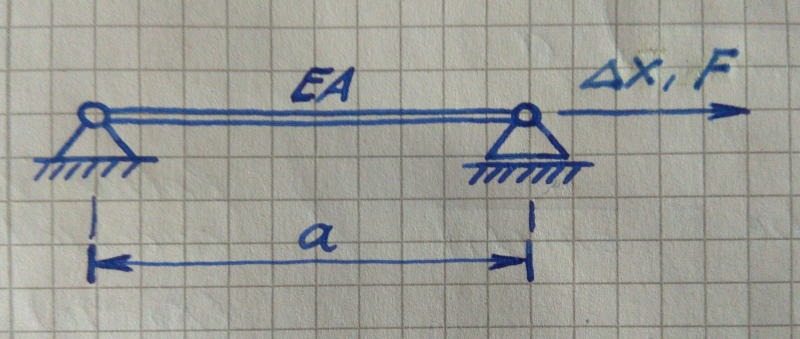
\includegraphics[width=0.4\textwidth]{figures/verification/linear-bar-truss-1.png}
\caption{Small deformation bar truss}
\label{fig:verification:linear-bar-truss-1}
\end{figure}

All displacements of the truss are assumed to be small, so any geometrically nonlinear effects can be neglected.
The relationship between force and displacement is found to be

$$
\Delta x = \frac{Fa}{EA}.
$$

\newpage
\subsection*{Linear bar truss (2)}

The bar shown in figure~\ref{fig:verification:linear-constraints} is fixed to the coordinate origin at one node, while the other node can slide along a line with angle $\alpha$.
A horizontal force $F_{x}$ is applied at this node.

\begin{figure}[H]
\centering
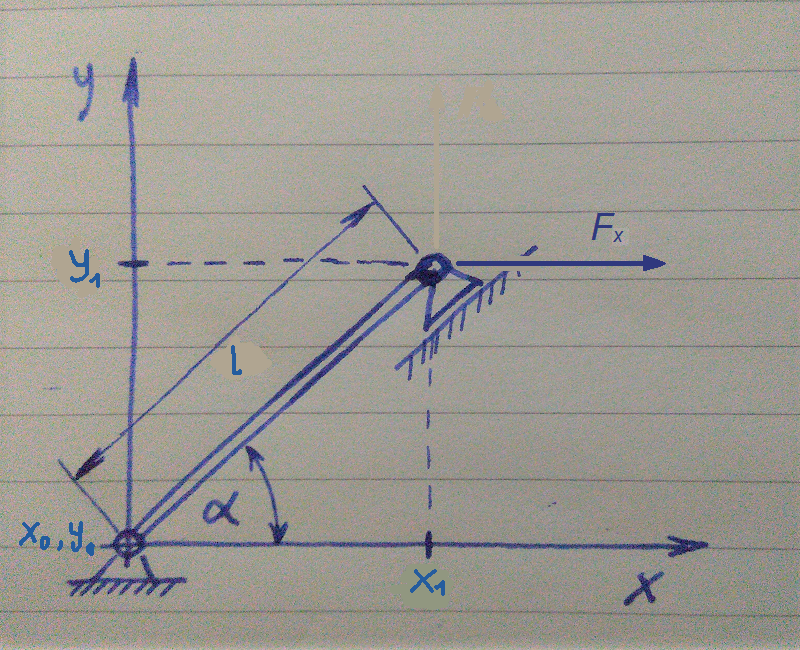
\includegraphics[width=0.4\textwidth]{figures/verification/linear-constraints.png}
\caption{Linearly constrained bar element}
\label{fig:verification:linear-constraints}
\end{figure}

The analytical relationships between the force $F$ in direction of the bar, its components $F_{x}$ and $F_{y}$ as well as the elongated length $l$ are
%
\begin{align*}
F &= EA\,\frac{l - l_{0}}{l_{0}} & F_{x} &= F\,\cos(\alpha) & F_{y} &= F\,\sin(\alpha)
\end{align*}
%
The kinematic constraints between $x_{1}$, $x_{1}$ and $l$, are
%
\begin{align*}
x_{1} &= l\,\cos(\alpha) & y_{1} &= l\,\sin(\alpha)
\end{align*}
%
The equation of motion of the unrestricted element, together with the kinematic constraints, are:

$$
\begin{bmatrix}
m_{00} & m_{01} & m_{02} & m_{03} \\
m_{10} & m_{11} & m_{12} & m_{13} \\
m_{20} & m_{21} & m_{22} & m_{23} \\
m_{30} & m_{31} & m_{32} & m_{33}
\end{bmatrix}
\begin{bmatrix}
\ddot{x}_{0} \\ \ddot{y}_{0} \\ \ddot{x}_{1} \\ \ddot{y}_{1}
\end{bmatrix}
+
\begin{bmatrix}
q_{0} \\ q_{1} \\ q_{2} \\ q_{3}
\end{bmatrix}
=
\begin{bmatrix}
p_{0} \\ p_{1} \\ p_{2} \\ p_{3}
\end{bmatrix}
,\quad
\begin{bmatrix}
x_{0} \\ y_{0} \\ x_{1} \\ y_{1}
\end{bmatrix}
=
\begin{bmatrix}
0 \\ 0 \\ \cos(\alpha) \\ \sin(\alpha)
\end{bmatrix}
\cdot l
$$

By applying the constraints to the equation of motion, we get a one-dimensional equation in terms of $l$ with the terms:
%
\begin{align*}
M &= m_{22}\cos(\alpha)^2 + (m_{23} + m_{32})\sin(\alpha)\cos(\alpha) + m_{33}\sin(\alpha)^2 \\
K &=  k_{22}\cos(\alpha)^2 + (k_{23} + k_{32})\sin(\alpha)\cos(\alpha) + k_{33}\sin(\alpha)^2 \\
Q &= q_{2}\cos(\alpha) + q_{3}\sin(\alpha) \\
P &= p_{2}\cos(\alpha) + p_{3}\sin(\alpha)
\end{align*}

\subsection*{Linear bar truss (3)}

This example was adapted from \cite{bib:tm2} (B6.4 on page 231), numerical values were added.

Given is a bar truss according to figure \ref{fig:verification:linear-bar-truss-2}.
The bars 1-2, 2-3 and 1-3 have a stiffness of $EA = 21000\,\unit{N}$ (steel bar of $1 \times 1\,\unit{cm}$) and bar 3-4 has a stiffness of $2EA$.
The distance $a$ is $1\,\unit{m}$.
The system is subjected to a relatively small force of $F = 10\,\unit{N}$.

\begin{figure}[H]
\centering
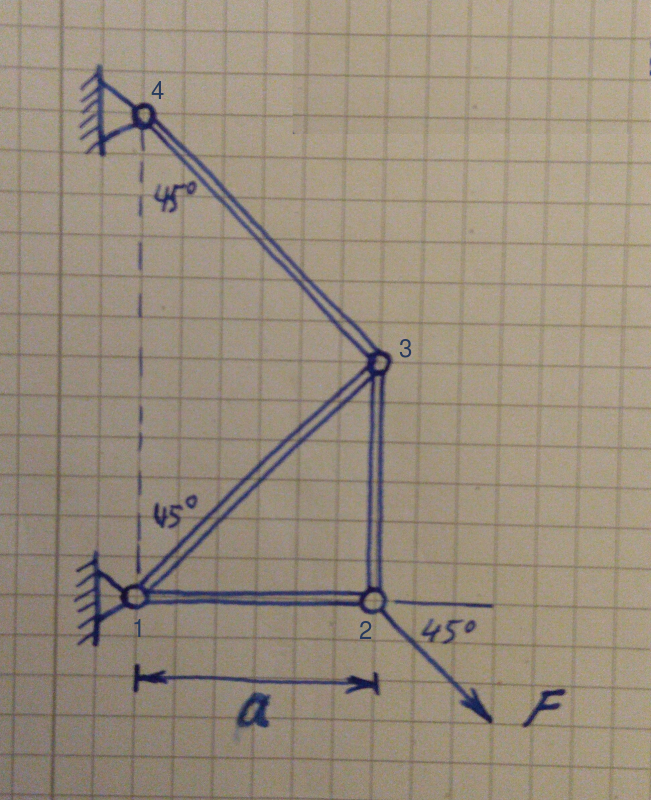
\includegraphics[width=0.3\textwidth]{figures/verification/linear-bar-truss-2.png}
\caption{Small deformation bar truss}
\label{fig:verification:linear-bar-truss-2}
\end{figure}


The task is to calculate the equilibrium displacements $\Delta x$ and $\Delta y$ of node 3.
All displacements of the truss are assumed to be small, so any geometrically nonlinear effects can be neglected.
According to \cite{bib:tm2} the solution is

$$
\Delta x = -\frac{1}{4}\frac{Fa}{EA},\quad \Delta y = -\frac{3}{4}\frac{Fa}{EA}.
$$

\subsection*{Linear bar truss (4)}

This example was adapted from \cite{bib:tm2} (B6.3 on page 230), numerical values were added.

Given is a bar truss according to figure \ref{fig:verification:linear-bar-truss-3} consisting of bars with a longitudinal stiffness of $EA = 21000\,\unit{N}$ (steel bar of $1 \times 1\,\unit{cm}$).
The distance $a$ is $1\,\unit{m}$.
The system is subjected to a relatively small force of $F = 10\,\unit{N}$.

\begin{figure}[H]
\centering
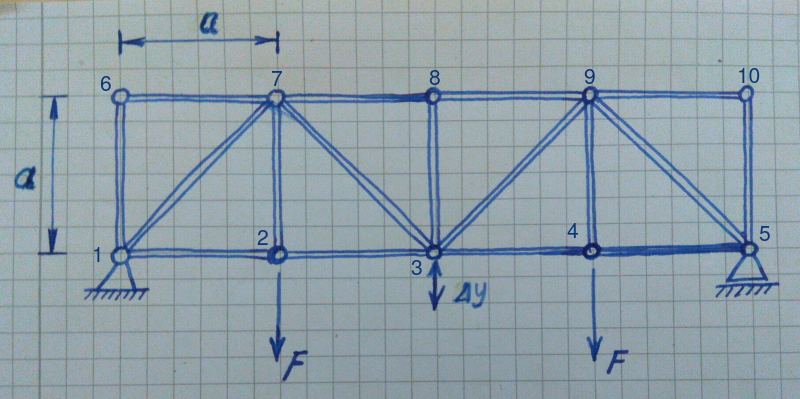
\includegraphics[width=0.5\textwidth]{figures/verification/linear-bar-truss-3.png}
\caption{Small deformation bar truss}
\label{fig:verification:linear-bar-truss-3}
\end{figure}

The task is to calculate the equilibrium displacement $\Delta y$ of the center node at the bottom.
All displacements of the truss are assumed to be small, so any geometrically nonlinear effects can be neglected.
According to \cite{bib:tm2} the solution is

$$
\Delta y = -\left(4 + 2\sqrt{2}\right)\frac{Fa}{EA}.
$$

\subsection*{Nonlinear bar truss (1)}

The bar truss shown in figure \ref{fig:verification:nonlinear-bar-truss-1} consists of a single bar with longitudinal stiffness $EA = 21000\,\unit{N}$.
The dimensions are $a = 1\,\unit{m}$ and $b = 0.1\,\unit{m}$.

\begin{figure}[H]
\centering
\includegraphics[width=0.3\textwidth]{figures/verification/nonlinear-bar-truss-1.png}
\caption{Large deformation bar truss}
\label{fig:verification:nonlinear-bar-truss-1}
\end{figure}

The task is to calculate the relationship between the position $y$ of the top right node and the applied force $F$ as well as the normal force $N$ in the bar.
Geometrical nonlinearity must be accounted for.
This system shows snap-through behaviour which tests the displacement control of the static solver.

\begin{align*}
l(y) &= \sqrt{a^2 + y^2} \\
N(y) &= EA\,\frac{l(y) - l(b)}{l(b)}, \\
F(y) &= \frac{y\,N(y)}{l(y)}.
\end{align*}

\newpage
\subsection*{Nonlinear bar truss (2)}

The bar truss shown in figure \ref{fig:verification:nonlinear-bar-truss-1} is sometimes referred to as the \textit{Von Mises Truss} and is commonly used to illustrate snap-through behaviour of nonlinear structures.
In this example the two bars have a longitudinal stiffness of~$EA = 21000\,\unit{N}$.
The dimensions are~$a = 0.4\,\unit{m}$,~$b = 0.6\,\unit{m}$ and~~$c = 0.1\,\unit{m}$.

\begin{figure}[H]
\centering
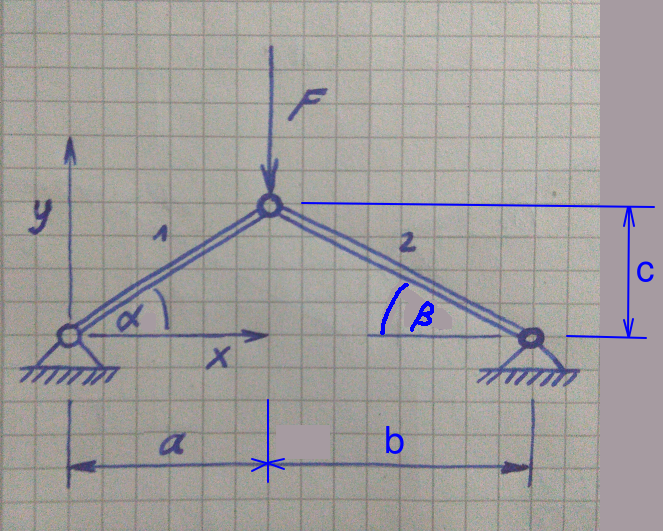
\includegraphics[width=0.3\textwidth]{figures/verification/nonlinear-bar-truss-2.png}
\caption{Large deformation bar truss}
\label{fig:verification:nonlinear-bar-truss-2}
\end{figure}

Lengths and angles of the two bars depending on the position $(x,\,y)$ of the top node:
%
\begin{align}
l_1(x,\,y) &= \sqrt{x^2 + y^2} \\
l_2(x,\,y) &= \sqrt{(a + b - x)^2 + y^2} \\
\alpha(x,\,y) &= \arctan \left( \frac{y}{x} \right) \\
\beta(x,\,y) &= \arctan \left( \frac{y}{a + b - x} \right)
\end{align}

From the lengths the normal forces in the bars are calculated as
%
\begin{align}
N_1(x,\,y) &= EA \cdot \frac{l_1(x,\,y) - l_1(x_0,\,y_0)}{l_1(x_0,\,y_0)}, \\
N_2(x,\,y) &= EA \cdot \frac{l_2(x,\,y) - l_2(x_0,\,y_0)}{l_2(x_0,\,y_0)}.
\end{align}

With the initial positions $x_0 = a$ and $y_0 = c$.
Finally, the equilibrium conditions in terms of the two normal forces $N_1$ and $N_2$ are
%
\begin{align}
-N_1 \cos{\alpha} + N_2 \cos{\beta} &= 0 \\
-N_1 \sin{\alpha} - N_2 \sin{\beta} &= F
\end{align}

Even though they can't be analytically solved for the displacements $x$ and $y$, we can still use these conditions to check whether the numerical solution of the problem satisfies them.

\newpage
\subsection*{Elastic catenary}

An elastic cable of length $l = 1.5\,\unit{m}$ is fixed between two points with horizontal distance $h = 1\,\unit{m}$ as shown in figure~\ref{fig:verification:cable-catenary}.
It is hanging freely under its own weight $\rho A = 1\,\unitfrac{kg}{m}$ and stiffness $EA = 10\,\unit{N}$.
The gravitaional acceleration is $g = 9.81\,\unitfrac{m}{s^2}$.

\begin{figure}[H]
\centering
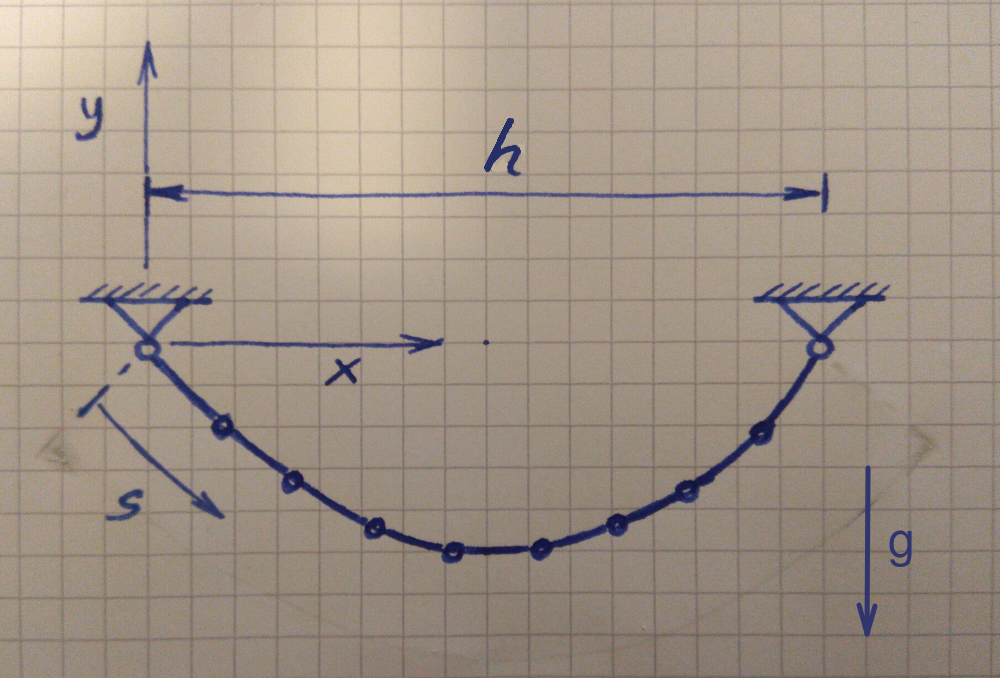
\includegraphics[width=0.3\textwidth]{figures/verification/cable-catenary.png}
\caption{Elastic cable hanging under its own weight}
\label{fig:verification:cable-catenary}
\end{figure}

The curve that such a cable assumes in static equilibrium is called \textit{elastic catenary}~\cite{bib:catenary} and can be expressed as
%
\begin{align}
x(s) &= c\,\arsinh \left(\frac{s - s_{0}}{c}\right) + c\,\frac{\rho g}{E}\,(s - s_{0}) + x_{0}, \\
y(s) &= \sqrt{c^2 + (s - s_{0})^2} + \frac{\rho g}{E}\,\frac{(s - s_{0})^2}{2} + y_{0},
\end{align}
%
where $s \in [0,\,l]$ is the natural length of the cable and $c$, $s_{0}$, $x_{0}$ and $y_{0}$ are constants that are determinied by the boundary conditions.
The normal force in the cable is given as

\begin{equation}
N(s) = \rho A\,g\,\sqrt{c^2 + (s - s_{0})^2}.
\end{equation}

The boundary conditions according to figure~\ref{fig:verification:cable-catenary} are
%
\begin{align}
x(0) &= 0: \quad x_{0} = c\,\arsinh \left(\frac{s_{0}}{c}\right) + c\,\frac{\rho g}{E}\,s_{0} \\
y(0) &= 0: \quad y_{0} = -\sqrt{c^2 + s_{0}^2} - \frac{\rho g}{E}\,\frac{s_{0}^2}{2} \\
y(l) &= 0: \quad s_{0} = \frac{l}{2} \\
x(l) &= h: \quad 2c\,\arsinh \left(\frac{l}{2c}\right) + c\,\frac{\rho g}{E}\,l - h = 0
\end{align}

The last equation for $c$ an only be solved numerically, which results in $c = 0.171344793374940\,\unit{m}$ and therefore $x_{0} = 0.5\,\unit{m}$ and $y_{0} = -1.045230003836251\,\unit{m}$.

% MATLAB code for numerical solution and verification
% =================================
%
% h = 1;
% l = 1.5;
% g = 9.81;
% 
% rA = 1.0;
% EA = 10.0;
% 
% c = fzero(@(x) 2*x*asinh(l/(2*x)) + x*rA*g/EA*l - h, 1);
% 
% s0 = l/2;
% x0 = c*asinh(s0/c) + c*rA*g/EA*s0;
% y0 = -sqrt(c^2 + s0^2) - rA*g/EA*s0^2/2;
% 
% s = linspace(0, l, 100);
% x = c*asinh((s - s0)/c) + c*rA*g/EA*(s - s0) + x0;
% y = sqrt(c^2 + (s - s0).^2) + rA*g/EA*(s - s0).^2/2 + y0;
% 
% plot(x, y);
% daspect([1 1 1])
% grid on;

\newpage
\subsection*{Linear beams}

The static solution of straight, geometrically linear cantilever beams with constant cross section are simple polynomial functions.
A single finite beam element with polynomial shape functions should also capture those solutions, provided that the order of the shape functions is at least as high as the order of the analytical solution.

\subsubsection*{Elongation}

TODO: Image, parameters

Clamping a linear beam on the left and subjecting it to a longitudinal force $Fx$ should result in the constant strain

\begin{equation}
\varepsilon(x) = \frac{F}{EA},
\end{equation}

a total elongation of the beam of

\begin{equation}
\Delta l = l\,\varepsilon,
\end{equation}

as well as zero transversal displacement and curvature.

\subsubsection*{Curvature}

TODO: Image, parameters

Clamping a linear beam on the left and subjecting it to a transversal force $Fy$ results in the displacement solution
%
\begin{align*}
w''(x) &= \frac{F}{EI}(l - x), \\
w'(x) &= \frac{F}{6EI}(6l - 3x)x, \\
w(x) &= \frac{F}{6EI}(3l - x)x^2
\end{align*}

The curvature of the beam, in geometrically linear analysis, is $\kappa(x) \approx w''(x)$.
The strain $\varepsilon(x)$ in this example is zero.

\newpage
\subsubsection*{Composite cross section}

The composite cross section in figure \ref{fig:verification:composite-section} was taken and slightly from an example in \cite{bib:tm2}.
It consists of 5 rectangular layers of equal height of $h = 8\,\unit{cm}$ and a width of $w = 40\,\unit{cm}$.
The material properties of the layers are given as $E_{c} = 10\,\unit{GPa}$ and $E_{s} = 5\,\unit{GPa}$.

\begin{figure}[H]
\centering
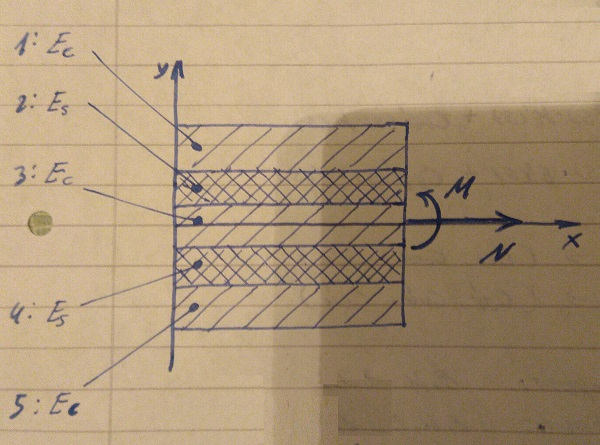
\includegraphics[width=0.6\textwidth]{figures/verification/composite-section}
\caption{Composite cross section of a beam with normal force $N$ and torque $M$}
\label{fig:verification:composite-section}
\end{figure}

The cross section is loaded by a compressive normal force $N = -500\,\unit{kNm}$ and a bending moment of $M = 60\,\unit{kNm}$.
Wanted is the distribution of strain and stress across the section.

In the original source the strains are given as $\varepsilon_{o} = -10.18 \cdot 10^{-4}$ at the top edge of the section and $\varepsilon_{u} = 2.38 \cdot 10^{-4}$ at the bottom edge, with a linear distribution inbetween due to the Bernoulli assumption.

Similarly, the stresses are given at the top and bottom of each layer as

\begin{tabular}{|c|c|c|}
\hline
Layer & Stress top [MPa] & Stress bottom [MPa] \\
\hline
1 & -10.18 & -7.66 \\
2 & -3.83 & -2.58 \\
3 & -5.16 & -2.64 \\
4 & -1.32 & -0.07 \\
5 & -0.14 & 2.38 \\
\hline
\end{tabular}

\newpage
\subsection*{Nonlinear beams}

Several reference beam problems are defined.
They have the following setup in common

\begin{itemize}
\item Planar (2D) problem
\item Beam fixed on the left and subjected to forces on the free end
\item Large displacements
\end{itemize}

The setup varies in the following aspects

\begin{itemize}
\item Initially straight vs curved beams
\item Constant vs tapered cross sections
\item Offset of the beam axis
\end{itemize}

The offset is defined by the parameter $p \in [-0.5,\,0.5]$ as shown in figure \ref{fig:verification:reference-beam-p}.

\begin{figure}[H]
\centering
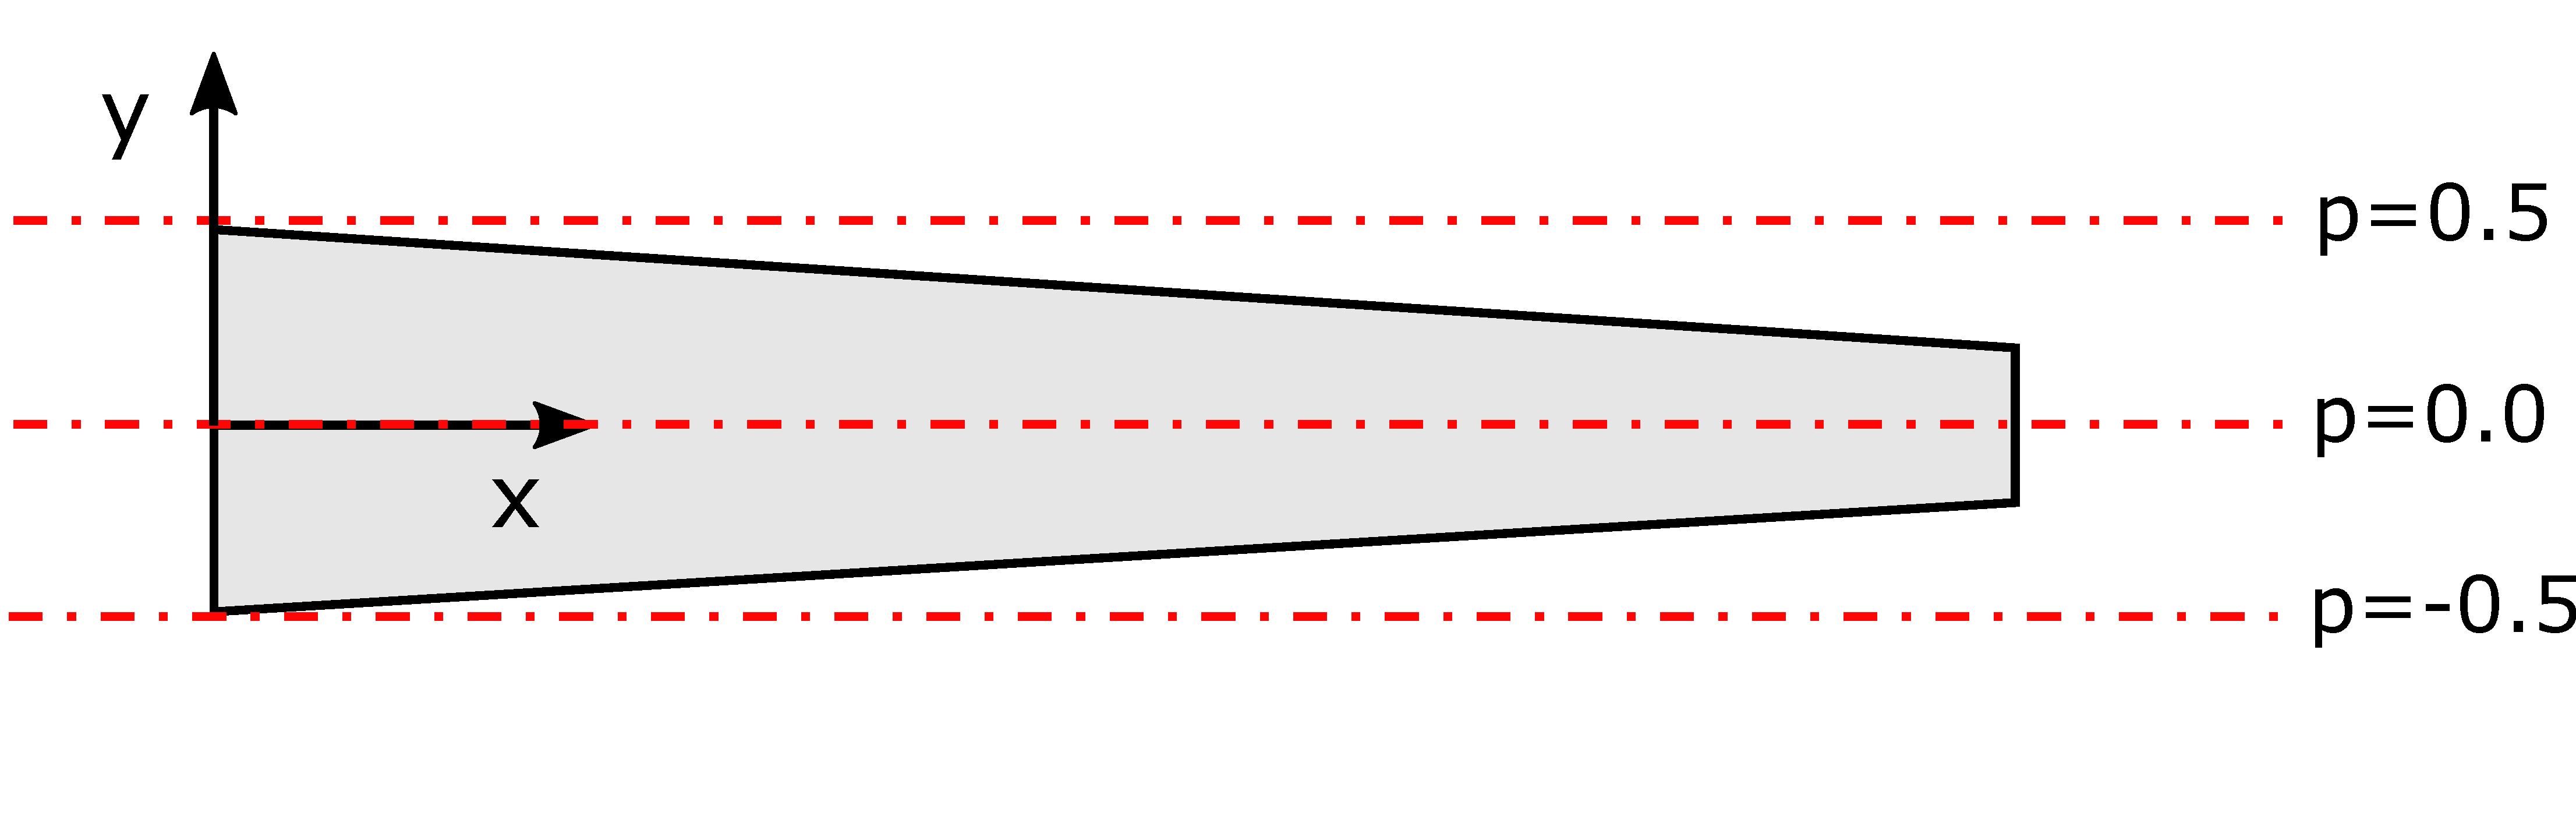
\includegraphics[width=0.8\textwidth]{figures/verification/reference-beam-p}
\captionof{figure}{Parameter $p$ for varying the offset of the beam's centerline}
\label{fig:verification:reference-beam-p}
\end{figure}

The results for $p = 0$ were calculated with Abaqus/CAE 2021 (Student Edition).
The models use 50 elements of type B23 (2-node cubic beam with no shear flexibility) and are solved with Nlgeom turned on in order to account for nonlinearity due to large displacements.

The results being calculated are the displacements $u_x$ and $u_y$ at 10 equal intervals over the beam length as well as the first 6 eigenfrequencies at the initial configuration.

Each of the reference beams is solved for the different offsets $p \in \{-0.5,\,-0.25,\,0.0,\,0.25,\,0.5\}$.
As the offset is only a geometric transformation, the deformation and dynamic behaviour of the beam itself has to be the same in all cases.
This can be checked in the following ways:

\begin{itemize}
\item Compare the nodal positions for each $p$ and check whether they have the correct distance and direction to each other (spaced by $0.25\,h$ and collinear).
\item Compare the eigenfrequencies for each $p$. They should be equal or very close.
\end{itemize}

The section's forces and bending moment can be calculated analytically for all reference beam by static balance with the tip forces $F_{x}$ and $F_{y}$.

\begin{align}
M(s) &= F_{y}\left(x(l) - x(s)\right) - F_{x}\left(y(l) - y(s)\right) \\
N(s) &= F_{x}\cos(\varphi(s)) + F_{y}\sin(\varphi(s)) \\
Q(s) &= F_{y}\cos(\varphi(s)) - F_{x}\sin(\varphi(s))
\end{align}

\newpage
\subsubsection*{Reference beam 1}

% Analytical eigenfrequencies, match the reference solution pretty well
% https://wandinger.userweb.mwn.de/LA_Elastodynamik_2/kap_3_balken.pdf
% TODO: Add to documentation of test cases
%
% double k1 = 1.8751*l;
% double k2 = 4.6941*l;
% double k3 = 7.8548*l;
% double k4 = 10.996*l;
% double k5 = (2*5 - 1)*M_PI/(2*l);
% double k6 = (2*6 - 1)*M_PI/(2*l);
%
% double f1 = k1*k1/(2*M_PI)*std::sqrt(Ckk(0)/rhoA(0));
% double f2 = k2*k2/(2*M_PI)*std::sqrt(Ckk(0)/rhoA(0));
% double f3 = k3*k3/(2*M_PI)*std::sqrt(Ckk(0)/rhoA(0));
% double f4 = k4*k4/(2*M_PI)*std::sqrt(Ckk(0)/rhoA(0));
% double f5 = k5*k5/(2*M_PI)*std::sqrt(Ckk(0)/rhoA(0));
% double f6 = k6*k6/(2*M_PI)*std::sqrt(Ckk(0)/rhoA(0));
%
% std::cout << f1 << ", " << f2 << ", " << f3 << ", " << f4 << ", " << f5 << ", " << f6 << std::endl;


% https://tex.stackexchange.com/a/6854
\begin{minipage}{\textwidth}
	\begin{minipage}[b]{0.7\textwidth}
		\centering
		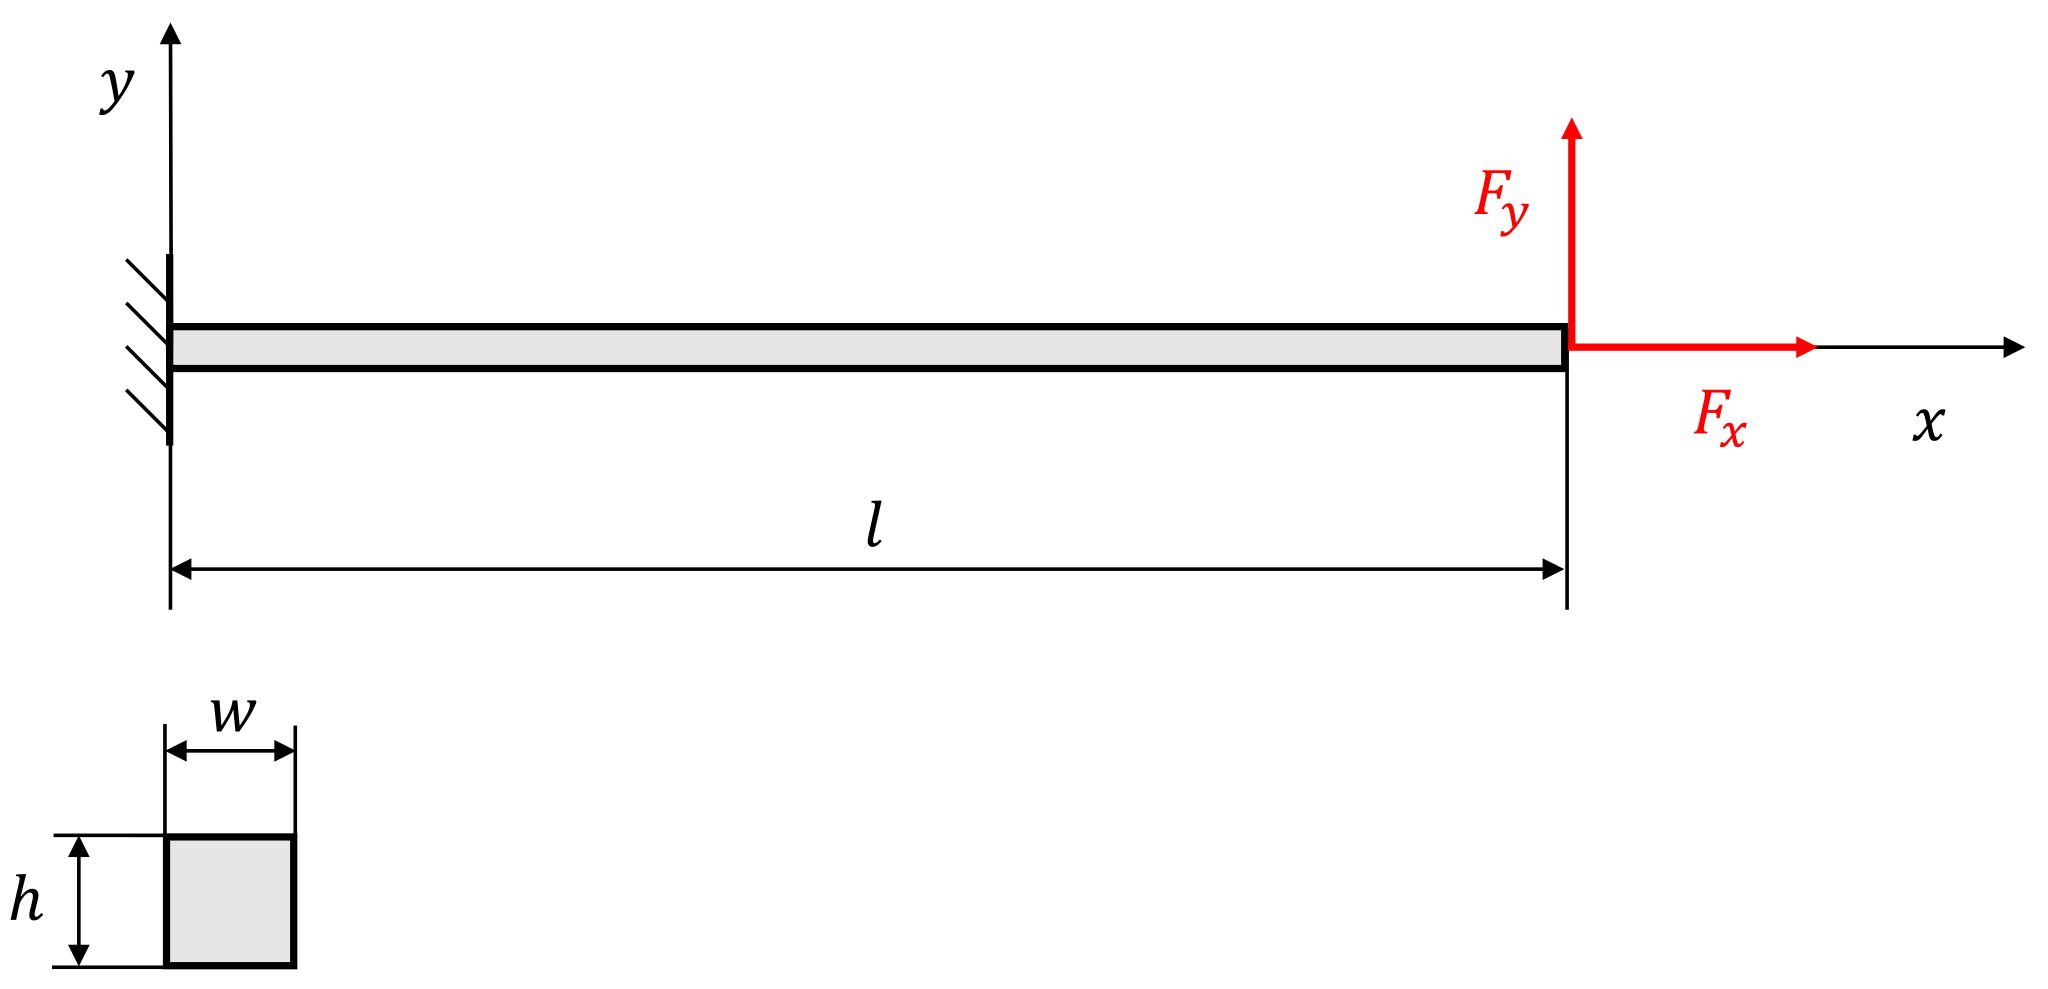
\includegraphics[width=\textwidth]{figures/verification/reference-beam-1}
		\captionof{figure}{Reference beam 1 (initially straight, constant cross section)}
	\end{minipage}
	\hfill
	\begin{minipage}[b]{0.29\textwidth}
		\centering
		\begin{tabular}{|cl|}
			\hline
			\multicolumn{2}{|c|}{Parameters} \\
			\hline
			$l$ & $\unit[1000]{mm}$ \\
			$w$ & $\unit[10]{mm}$ \\
			$h$ & $\unit[10]{mm}$ \\
			$E$ & $\unit[210e9]{Pa}$ \\
			$\nu$ & $0.3$ \\
			$\rho$ & $\unitfrac[7850]{kg}{m^3}$ \\
			$F_x$ & $\unit[-200]{N}$ \\
			$F_y$ & $\unit[200]{N}$ \\
			\hline
		\end{tabular}
		\captionof{table}{Parameters for reference beam 1}
	\end{minipage}
\end{minipage}

\begin{table}[H]
\begin{tabular}{ll}
\hline
$u_x$ [m] & $u_y$ [m] \\
\hline
-6.26757e-34 & -9.52773e-36 \\
-0.000364492 & 0.00738275 \\
-0.00270887 & 0.0285538 \\
-0.00847269 & 0.0618318 \\
-0.0185084 & 0.105388 \\
-0.0331319 & 0.157389 \\
-0.0522044 & 0.216094 \\
-0.0752253 & 0.279902 \\
-0.101423 & 0.347369 \\
-0.129836 & 0.417189 \\
-0.159385 & 0.488158 \\
\hline
\end{tabular}
\begin{tabular}{ll}
\hline
$n$ & $f$ [Hz] \\
\hline
1 & 8.3552 \\
2 & 52.361 \\
3 & 146.61 \\
4 & 287.30 \\
5 & 474.93 \\
6 & 709.47 \\
\hline
\end{tabular}
\caption{Results Beam 1}
\end{table}

% Cross-verification:
% The analytical eigenfrequencies for this case match the reference solution pretty well
% https://wandinger.userweb.mwn.de/LA_Elastodynamik_2/kap_3_balken.pdf
%
% double k1 = 1.8751*l;
% double k2 = 4.6941*l;
% double k3 = 7.8548*l;
% double k4 = 10.996*l;
% double k5 = (2*5 - 1)*M_PI/(2*l);
% double k6 = (2*6 - 1)*M_PI/(2*l);
%
% double f1 = k1*k1/(2*M_PI)*std::sqrt(EI/rhoA);
% double f2 = k2*k2/(2*M_PI)*std::sqrt(EI/rhoA);
% double f3 = k3*k3/(2*M_PI)*std::sqrt(EI/rhoA);
% double f4 = k4*k4/(2*M_PI)*std::sqrt(EI/rhoA);
% double f5 = k5*k5/(2*M_PI)*std::sqrt(EI/rhoA);
% double f6 = k6*k6/(2*M_PI)*std::sqrt(EI/rhoA);
%
% std::cout << f1 << ", " << f2 << ", " << f3 << ", " << f4 << ", " << f5 << ", " << f6 << std::endl;

\newpage
\subsubsection*{Reference beam 2}

% https://tex.stackexchange.com/a/6854
\begin{minipage}{\textwidth}
	\begin{minipage}[b]{0.7\textwidth}
		\centering
		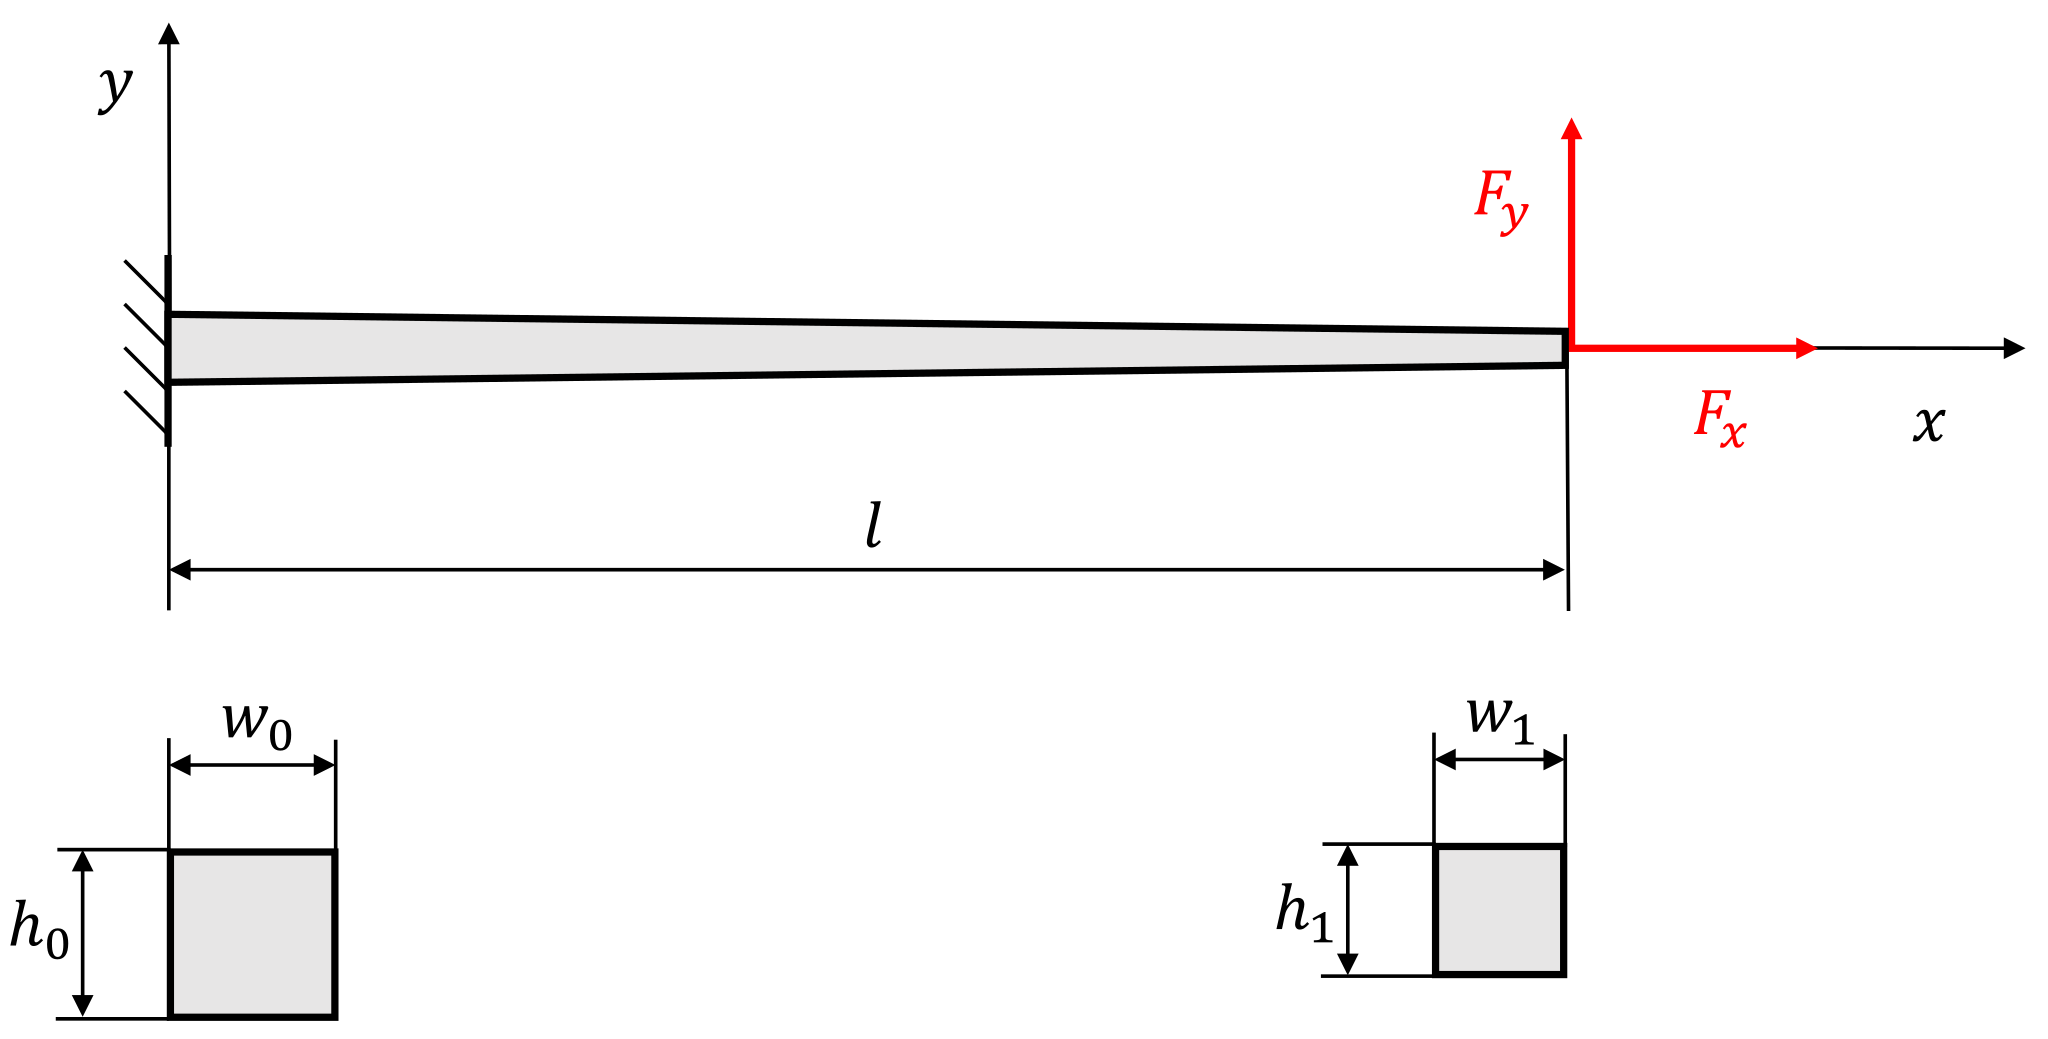
\includegraphics[width=\textwidth]{figures/verification/reference-beam-2}
		\captionof{figure}{Reference beam 2 (initially straight, tapered cross section)}
	\end{minipage}
	\hfill
	\begin{minipage}[b]{0.29\textwidth}
		\centering
		\begin{tabular}{|cl|}
			\hline
			\multicolumn{2}{|c|}{Parameters} \\
			\hline
			$l$ & $\unit[1000]{mm}$ \\
			$w_0$ & $\unit[10]{mm}$ \\
			$h_0$ & $\unit[10]{mm}$ \\
			$w_1$ & $\unit[5]{mm}$ \\
			$h_1$ & $\unit[5]{mm}$ \\
			$E$ & $\unit[210e9]{Pa}$ \\
			$\nu$ & $0.3$ \\
			$\rho$ & $\unitfrac[7850]{kg}{m^3}$ \\
			$F_x$ & $\unit[-100]{N}$ \\
			$F_y$ & $\unit[100]{N}$ \\
			\hline
		\end{tabular}
		\captionof{table}{Parameters for reference beam 2}
	\end{minipage}
\end{minipage}

\begin{table}[H]
\begin{tabular}{ll}
\hline
$u_x$ [m] & $u_y$ [m] \\
\hline
-1.5028E-34 & -1.10343E-36 \\
-0.000100427 & 0.0038425 \\
-0.000873697 & 0.0159811 \\
-0.00322521 & 0.0373441 \\
-0.0083509 & 0.068785 \\
-0.0177466 & 0.110957 \\
-0.0331446 & 0.164138 \\
-0.0563114 & 0.228025 \\
-0.0886096 & 0.301526 \\
-0.130185 & 0.382624 \\
-0.178556 & 0.468253\\
\hline
\end{tabular}
\begin{tabular}{ll}
\hline
$n$ & $f$ [Hz] \\
\hline
1 & 10.988 \\
2 & 46.438 \\
3 & 115.40 \\
4 & 218.11 \\
5 & 354.89 \\
6 & 525.78 \\
\hline
\end{tabular}
\caption{Results Beam 2}
\end{table}

\newpage
\subsubsection*{Reference beam 3}

% https://tex.stackexchange.com/a/6854
\begin{minipage}{\textwidth}
	\begin{minipage}[b]{0.7\textwidth}
		\centering
		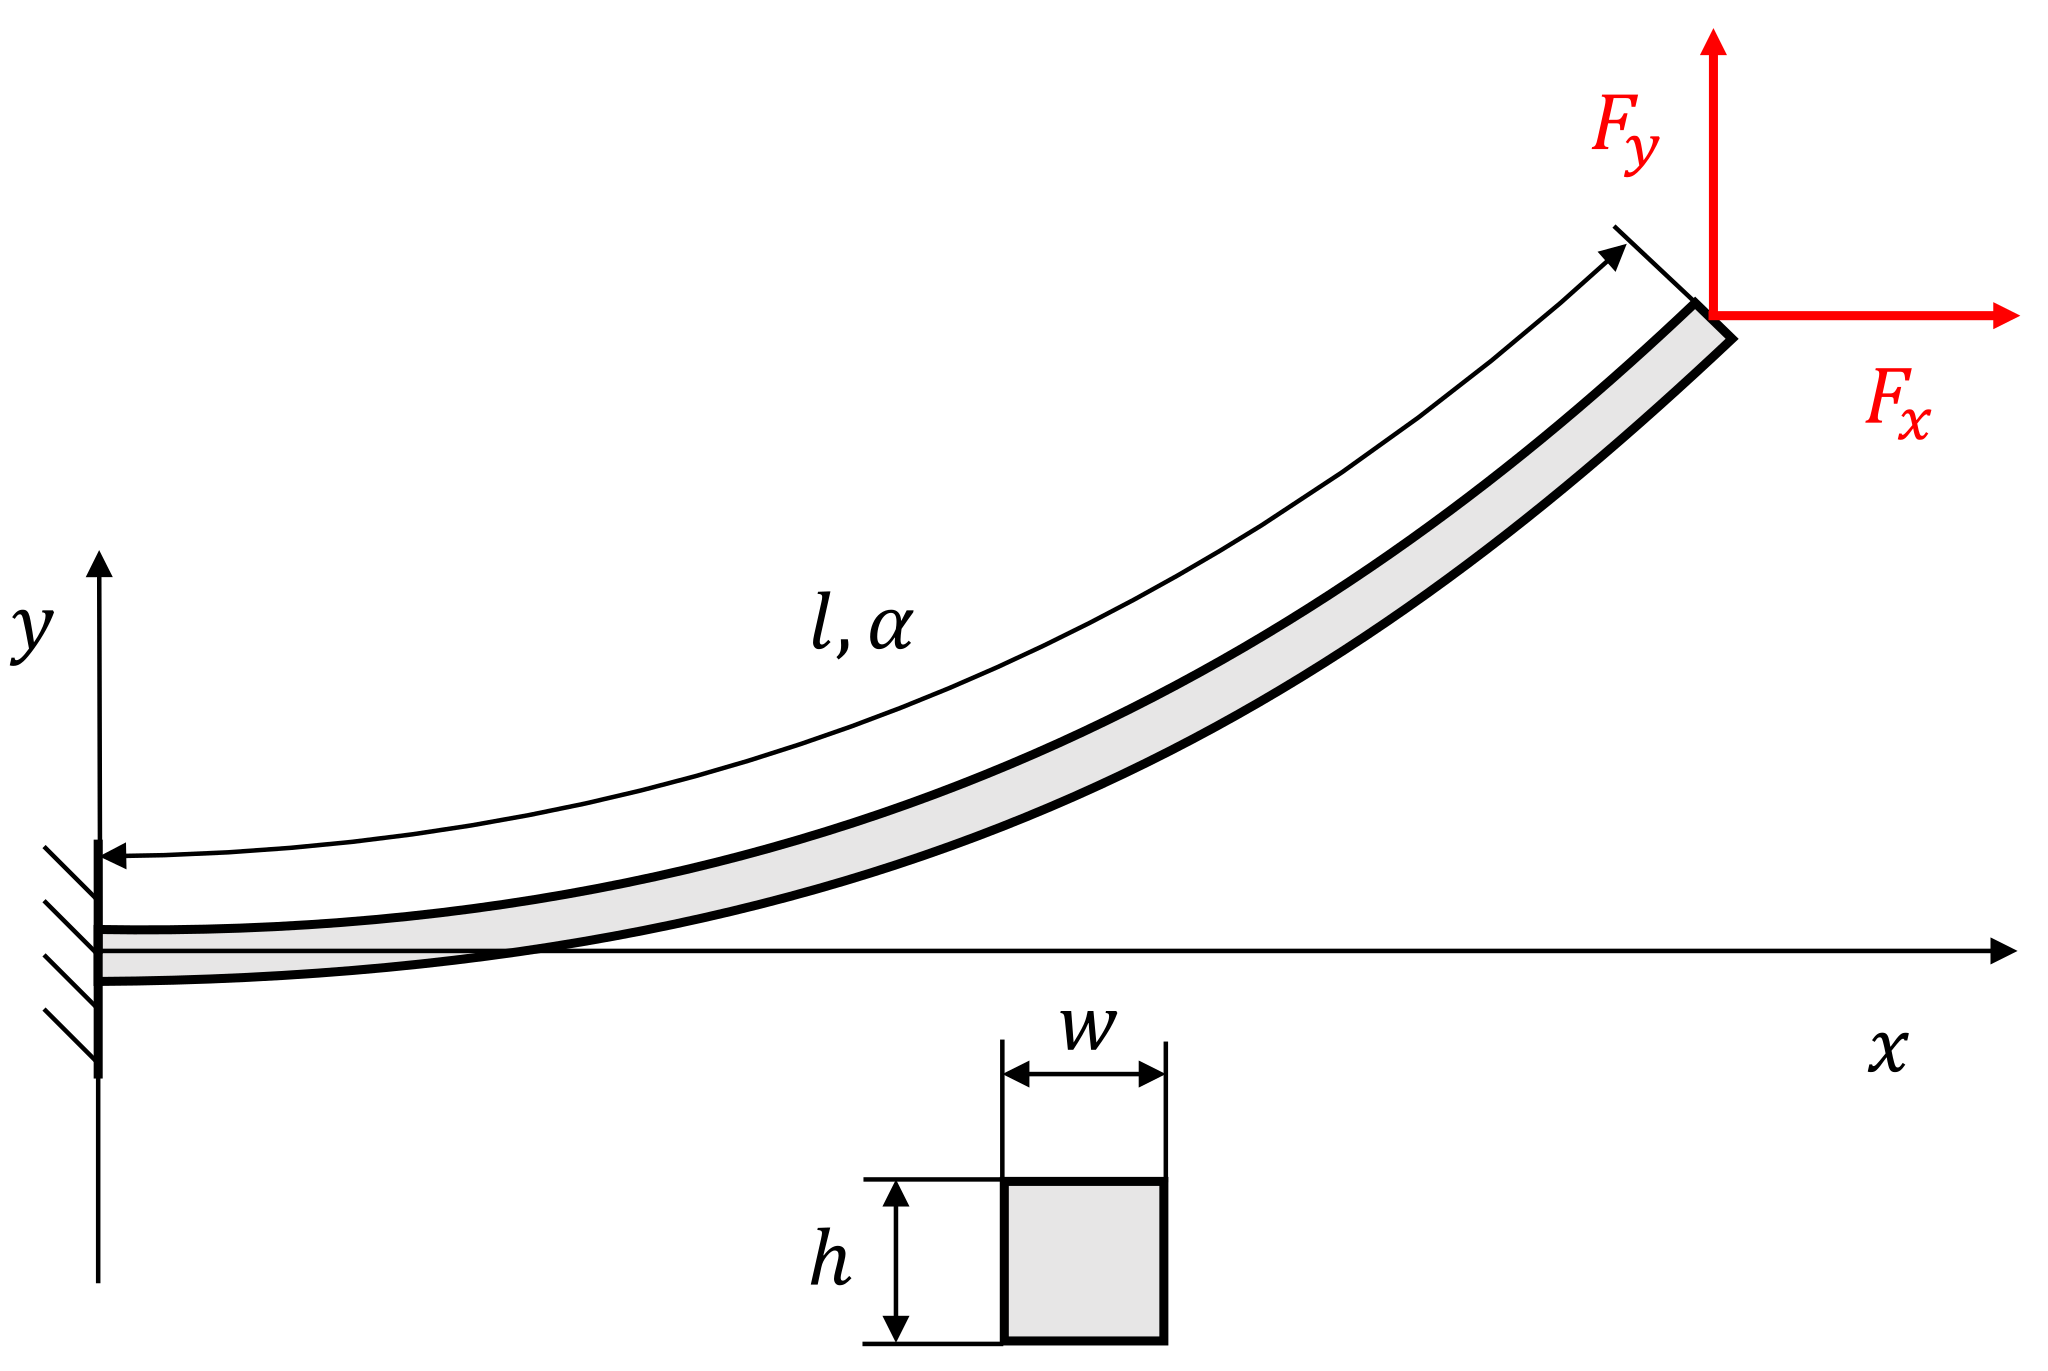
\includegraphics[width=0.8\textwidth]{figures/verification/reference-beam-3}
		\captionof{figure}{Reference beam 3 (circular arc, constant cross section)}
	\end{minipage}
	\hfill
	\begin{minipage}[b]{0.29\textwidth}
		\centering
		\begin{tabular}{|cl|}
			\hline
			\multicolumn{2}{|c|}{Parameters} \\
			\hline
			$l$ & $\unit[1000]{mm}$ \\
			$\alpha$ & $\unit[45]{^\circ}$ \\
			$(r)$ & $\unit[1273.24]{mm}$ \\
			$w$ & $\unit[10]{mm}$ \\
			$h$ & $\unit[10]{mm}$ \\
			$E$ & $\unit[210e9]{Pa}$ \\
			$\nu$ & $0.3$ \\
			$\rho$ & $\unitfrac[7850]{kg}{m^3}$ \\
			$F_x$ & $\unit[-200]{N}$ \\
			$F_y$ & $\unit[200]{N}$ \\
			\hline
		\end{tabular}
		\captionof{table}{Parameters for reference beam 3}
	\end{minipage}
\end{minipage}

\begin{table}[H]
\begin{tabular}{ll}
\hline
$u_x$ [m] & $u_y$ [m] \\
\hline
-2.09171E-33 & -4.41331E-35 \\
-0.000703401 & 0.00705204 \\
-0.00528883 & 0.026883 \\
-0.016655 & 0.0569289 \\
-0.0365555 & 0.0942108 \\
-0.0656897 & 0.135753 \\
-0.103887 & 0.178851 \\
-0.150332 & 0.221234 \\
-0.203777 & 0.261128 \\
-0.262739 & 0.297265 \\
-0.32561 & 0.328816 \\
\hline
\end{tabular}
\begin{tabular}{ll}
\hline
$n$ & $f$ [Hz] \\
\hline
1 & 8.4604 \\
2 & 49.038 \\
3 & 142.75 \\
4 & 283.14 \\
5 & 470.47 \\
6 & 704.52 \\
\hline
\end{tabular}
\caption{Results Beam 3}
\end{table}

\newpage
\subsubsection*{Reference beam 4}

% https://tex.stackexchange.com/a/6854
\begin{minipage}{\textwidth}
	\begin{minipage}[b]{0.7\textwidth}
		\centering
		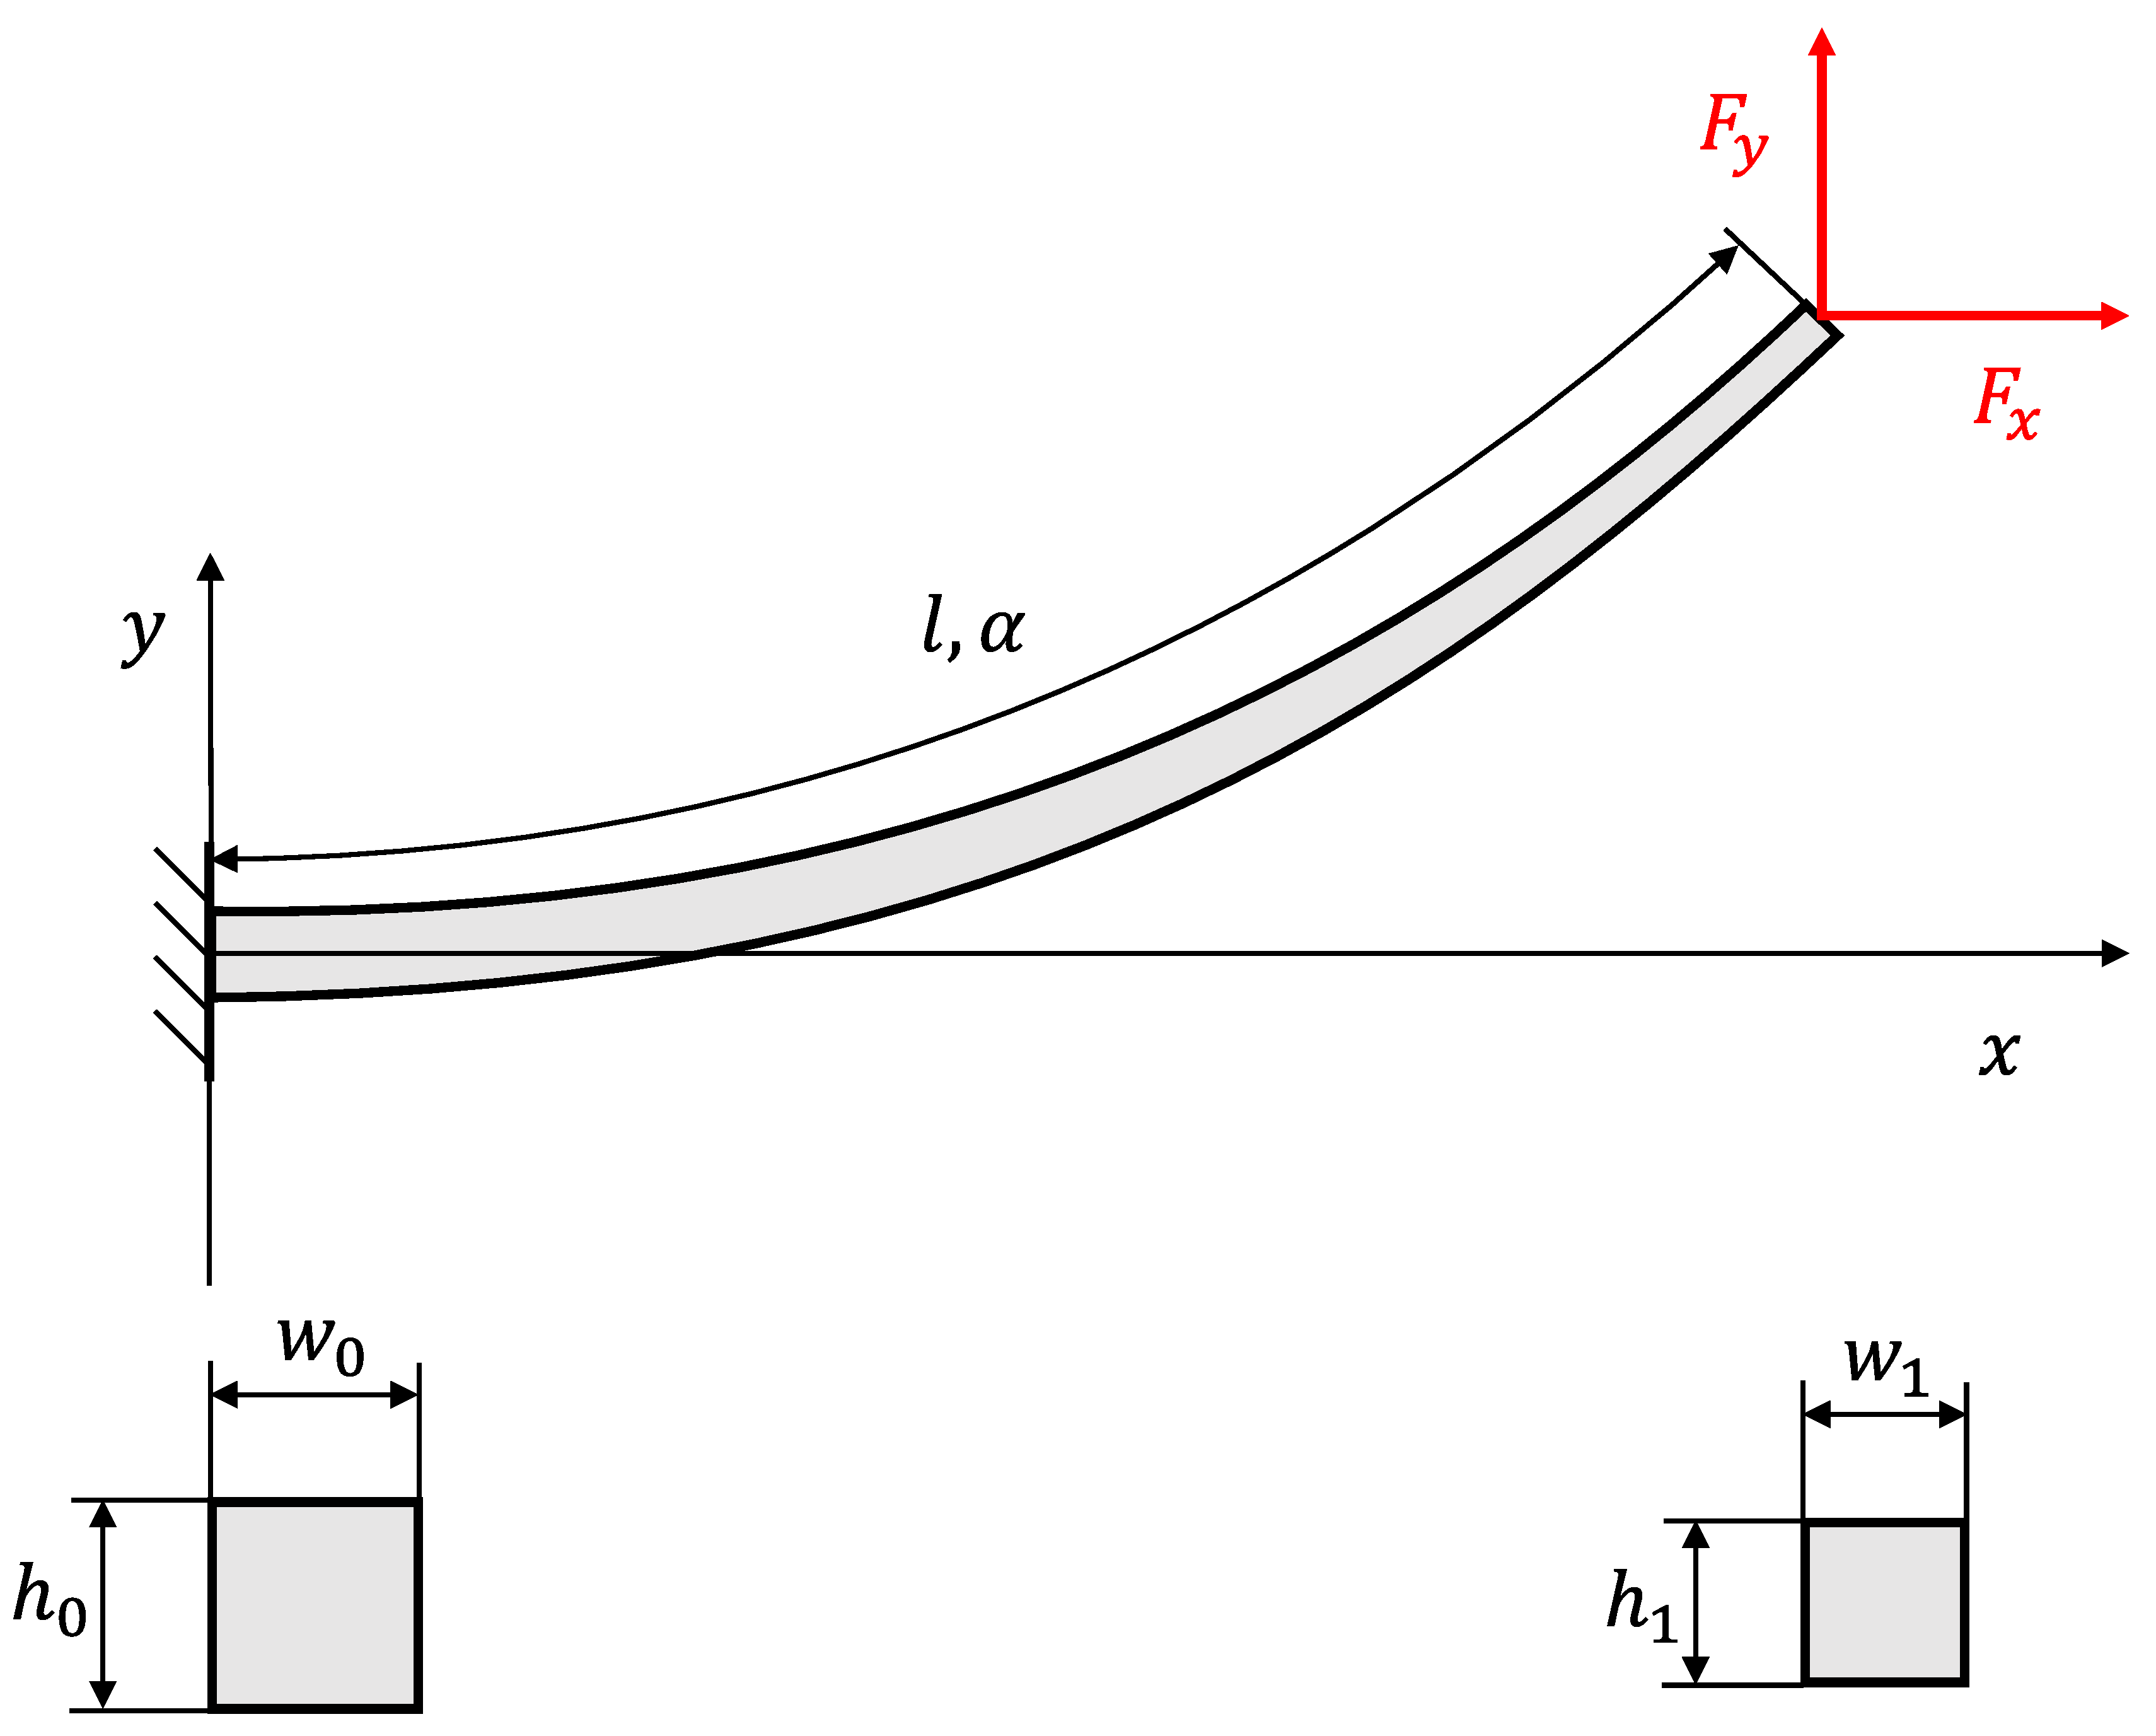
\includegraphics[width=0.8\textwidth]{figures/verification/reference-beam-4}
		\captionof{figure}{Reference beam 4 (circular arc, tapered cross section)}
	\end{minipage}
	\hfill
	\begin{minipage}[b]{0.29\textwidth}
		\centering
		\begin{tabular}{|cl|}
			\hline
			\multicolumn{2}{|c|}{Parameters} \\
			\hline
			$l$ & $\unit[1000]{mm}$ \\
			$\alpha$ & $\unit[45]{^\circ}$ \\
			$(r)$ & $\unit[1273.24]{mm}$ \\
			$w_0$ & $\unit[10]{mm}$ \\
			$h_0$ & $\unit[10]{mm}$ \\
			$w_1$ & $\unit[5]{mm}$ \\
			$h_1$ & $\unit[5]{mm}$ \\
			$E$ & $\unit[210e9]{Pa}$ \\
			$\nu$ & $0.3$ \\
			$\rho$ & $\unitfrac[7850]{kg}{m^3}$ \\
			$F_x$ & $\unit[-100]{N}$ \\
			$F_y$ & $\unit[100]{N}$ \\
			\hline
		\end{tabular}
		\captionof{table}{Parameters for reference beam 4}
	\end{minipage}
\end{minipage}

\begin{table}[H]
\begin{tabular}{ll}
\hline
$u_x$ [m] & $u_y$ [m] \\
\hline
-5.18203E-34 & -7.16919E-36 \\
-0.000284819 & 0.00366578 \\
-0.00239457 & 0.0150587 \\
-0.00846134 & 0.0344658 \\
-0.0208599 & 0.0616169 \\
-0.0420197 & 0.095539 \\
-0.0741302 & 0.134475 \\
-0.118746 & 0.175933 \\
-0.176322 & 0.216937 \\
-0.245706 & 0.254526 \\
-0.323543 & 0.286515 \\
\hline
\end{tabular}
\begin{tabular}{ll}
\hline
$n$ & $f$ [Hz] \\
\hline
1 & 11.110 \\
2 & 44.670 \\
3 & 113.23 \\
4 & 215.64 \\
5 & 352.29 \\
6 & 523.04 \\
\hline
\end{tabular}
\caption{Results Beam 4}
\end{table}

\newpage
\section{Bow limb}

After having performed a static simulation of a bow, there are various things that can be checked in order to verify that the system is indeed in static equilibrium.

\begin{figure}[H]
\centering
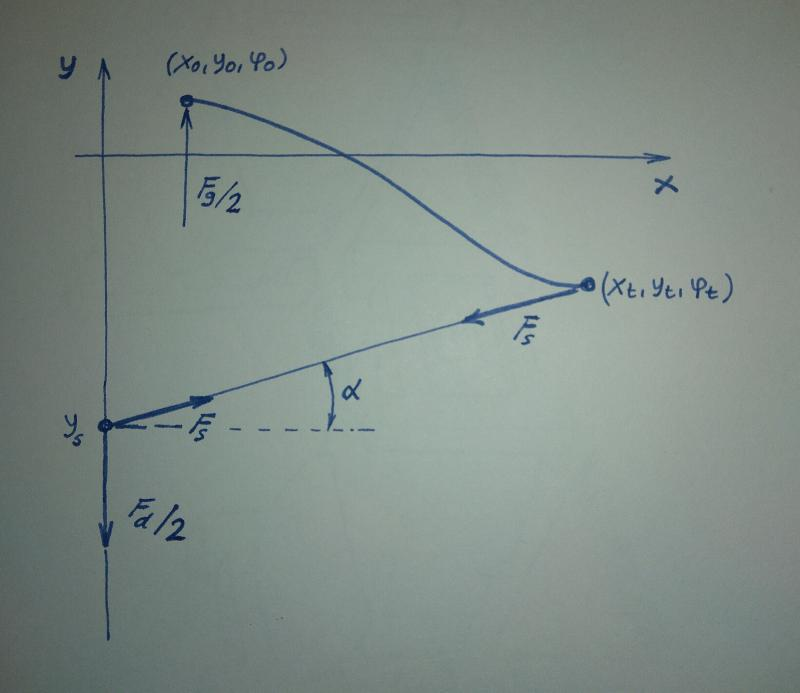
\includegraphics[width=0.6\textwidth]{figures/verification/bow-static-forces}
\captionof{figure}{Static equilibrium of a bow limb without recurve}
\label{fig:verification:bow-static-forces}
\end{figure}

\subsection*{String force}

If we balance the draw force $F_d$ and the string force $F_s$ at the center of the string, we get the following equilibrium condition in the $y$ direction,

\begin{equation}
F_d = 2F_s\,\sin(\alpha),\quad \alpha = \arctan\left(\frac{y_t - y_s}{x_t}\right).
\end{equation}

with the string angle $\alpha$ being computed from the limb tip position (only for non-recurve bows).
This can be used to verify that draw force and string force are consistent with each other.

\subsection*{Grip force}

Balancing the forces on the whole bow in the $y$ direction leads to $F_g = F_d$, i.e. the grip force must be equal to the draw force in the static case.

\subsection*{Section forces}

The string exerts a force on the limb tip with the two components

\begin{align}
F_x = -F_s\,\cos(\alpha), \\
F_y = -F_s\,\sin(\alpha).
\end{align}

As in the previous static beam tests [TODO: Reference], the cross section forces ($N$, $M$, $Q$) of the limb must be in equilibrium with this applied force.

\subsection*{Drawing work}

The change in potential energy of limbs and string as the bow is drawn must be equal to the work performed by the draw force over the draw length, computed as the numerical integral of the force-draw curve.



\newpage
\section{Dynamics}

\subsection*{Linear Mass-Spring-Damper System}

The linear $n$ degree of freedom system shown in figure~\ref{fig:verification:linear-fmd} consists of a series of equal masses $m$, connected by parallel combinations of springs with stiffness $k$ and dampers with damping coefficient $d$.

\begin{figure}[h]
\centering
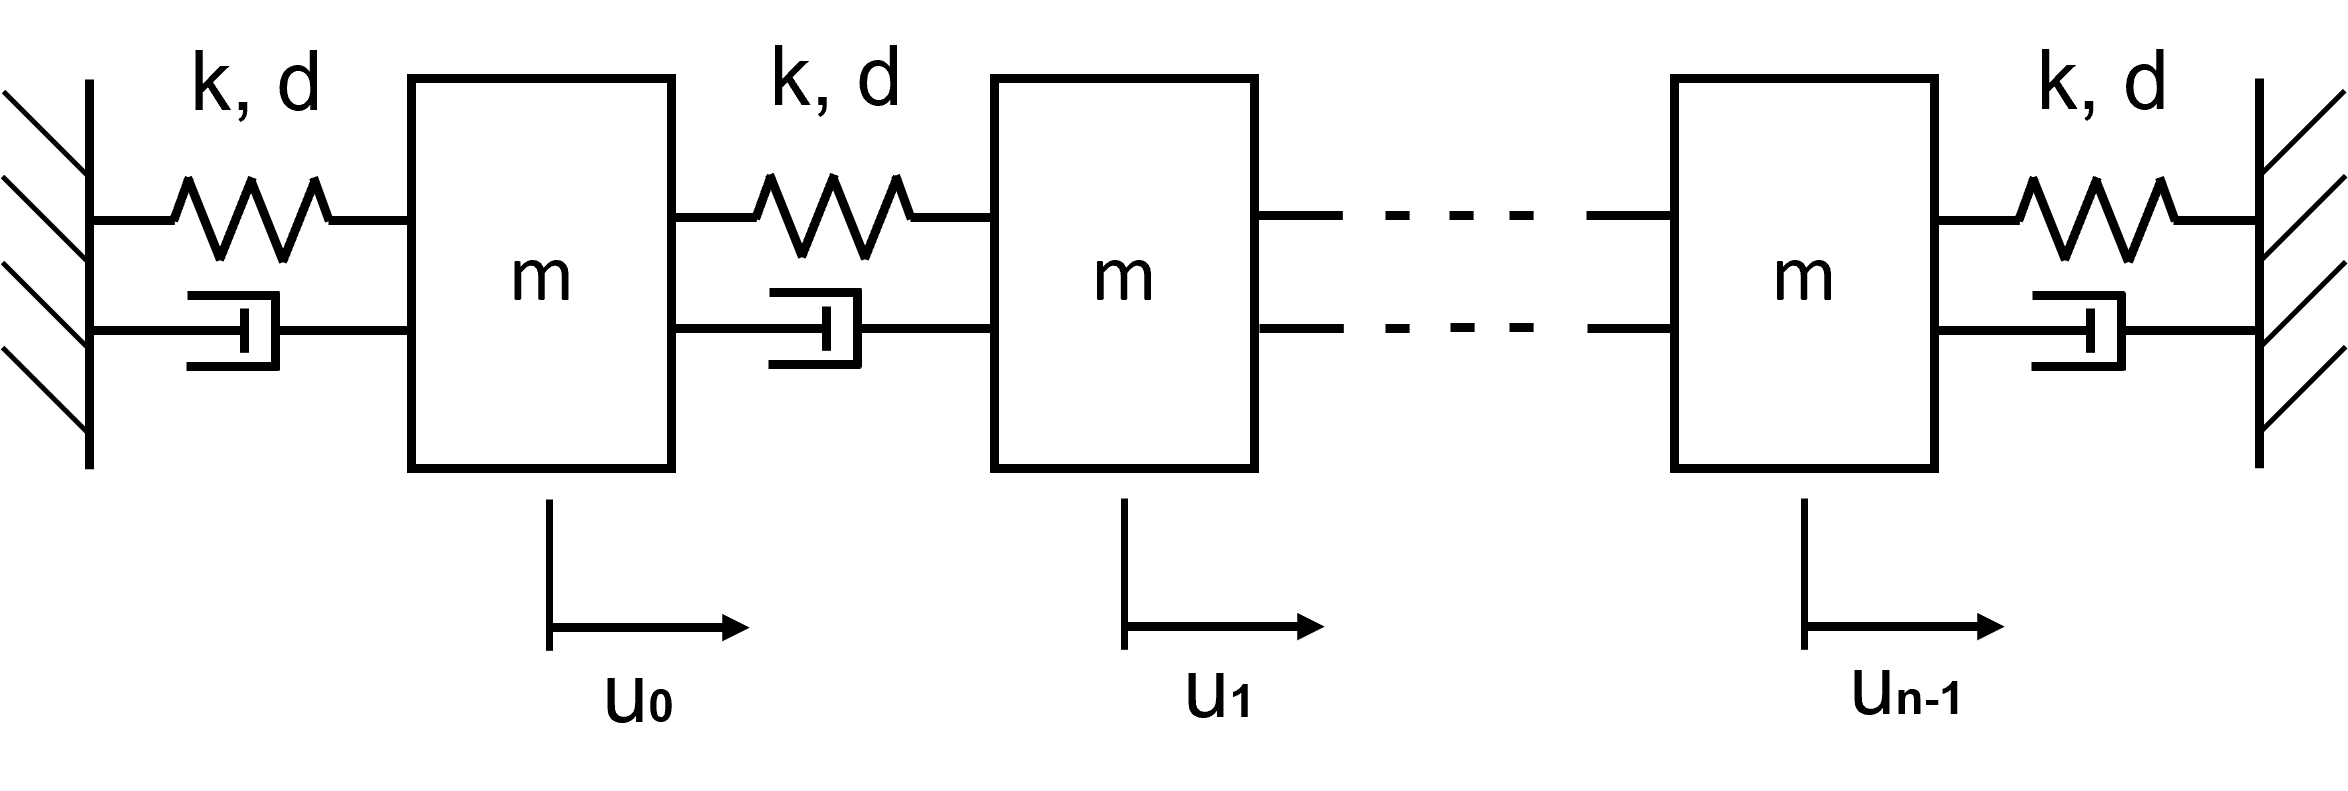
\includegraphics[width=0.6\textwidth]{figures/verification/mass-spring-damper}
\caption{Simple linear dynamical system with $n$ degrees of freedom}
\label{fig:verification:linear-fmd}
\end{figure}

The displacement vector $\boldsymbol{u}(t)$ consists of the horizontal displacements of the masses while a constant force $\boldsymbol{P}$ is applied to the system.
The equation of motion takes the form

\begin{equation}
\boldsymbol{M}\ddot{\boldsymbol{u}}(t) + \boldsymbol{D}\dot{\boldsymbol{u}}(t) + \boldsymbol{K}\boldsymbol{u}(t) = \boldsymbol{p}(t) \label{eq:verification:linear-fmd}
\end{equation}

where the mass-, damping- and stiffness matrices for this configuration can be derived as

\begin{align}
\boldsymbol{M} =
\begin{bmatrix}
m \\
& \ddots \\
&& m \\
&&& \ddots \\
&&&& m
\end{bmatrix}
 \
\boldsymbol{D} =
\begin{bmatrix}
2d & -d \\
& \ddots \\
& -d & 2d & -d \\
&&& \ddots \\
&&& -d & 2d
\end{bmatrix}
 \
\boldsymbol{K} =
\begin{bmatrix}
2k & -k \\
& \ddots \\
& -k & 2k & -k \\
&&& \ddots \\
&&& -k & 2k
\end{bmatrix}
\end{align}

The goal is to determine the motion of the system with arbitrary initial displacements and velocities as well as a harmonic excitation with frequency $\Omega$ ,
%
\begin{align}
\boldsymbol{u}(0) = \boldsymbol{u}_{0},\quad \dot{\boldsymbol{u}}(0) = \boldsymbol{v}_{0},\quad \boldsymbol{p}(t) = \boldsymbol{p}_{0}\cos(\Omega\,t)
\end{align}

Since (\ref{eq:verification:linear-fmd}) is a linear differential equation, we can solve it analytically to get reference solutions for our numeric integration algorithm.
As a first step we transformation (\ref{eq:verification:linear-fmd}) into a first-order system of the form $\dot{\boldsymbol{x}}(t) = \boldsymbol{A}\,\boldsymbol{x}(t) + \boldsymbol{b}(t)$:

\begin{equation}
\underbrace{
\begin{bmatrix} \dot{\boldsymbol{u}}(t) \\ \ddot{\boldsymbol{u}}(t) \end{bmatrix}
}_{\dot{\boldsymbol{x}}(t)}
=
\underbrace{
\begin{bmatrix}
\boldsymbol{0} & \boldsymbol{I} \\
-\boldsymbol{M}^{-1}\boldsymbol{K} & -\boldsymbol{M}^{-1}\boldsymbol{D}
\end{bmatrix}
}_{\boldsymbol{A}}
\underbrace{
\begin{bmatrix} \boldsymbol{u} \\ \dot{\boldsymbol{u}} \end{bmatrix}
}_{\boldsymbol{x}(t)}
+
\underbrace{
\begin{bmatrix}
\boldsymbol{0} \\
\boldsymbol{M}^{-1}\boldsymbol{p}(t)
\end{bmatrix}
}_{\boldsymbol{b}(t)}
\end{equation}

We also note that $\boldsymbol{b}(t)$ takes the form $\boldsymbol{b}(t) = \boldsymbol{b}_{0}\cos(\Omega\,t)$ with $\boldsymbol{b}_{0} = \begin{bmatrix}
\boldsymbol{0}, & \boldsymbol{M}^{-1}\boldsymbol{p}_{0}
\end{bmatrix}^\intercal$.
Using Euler's formula $e^{\rm{i}\Omega t} = \cos(\Omega t) + \rm{i}\cdot\sin(\Omega t)$ we rewrite this in terms of a complex exponential function as

\begin{equation}
\boldsymbol{b}(t) = \operatorname{Re}\left\{\boldsymbol{b}_{0}\,e^{\rm{i}\Omega t}\right\}.
\end{equation}

The solution of the initial value problem with $\boldsymbol{x}(0) = \boldsymbol{x}_{0}$, using the matrix exponential function $\boldsymbol{\phi}(t) = e^{\boldsymbol{A}t}$, can be written as

\begin{align}
\boldsymbol{x}(t) &= \boldsymbol{\phi}(t)\,\boldsymbol{x}_{0} + \int_{0}^{t} \boldsymbol{\phi}(t - \tau)\,\boldsymbol{b}(\tau)\,d\tau \\
&= \boldsymbol{\phi}(t)\,\boldsymbol{x}_{0} + \int_{0}^{t} \boldsymbol{\phi}(t - \tau)\,\operatorname{Re}\left\{\boldsymbol{b}_{0}\,e^{\rm{i}\Omega \tau}\right\}\,d\tau \\
&= \boldsymbol{\phi}(t)\,\boldsymbol{x}_{0} + \operatorname{Re}\bigg\{\underbrace{\int_{0}^{t} \boldsymbol{\phi}(t - \tau)\,\boldsymbol{b}_{0}\,e^{\rm{i}\Omega \tau}\,d\tau}_{\boldsymbol{x}^{*}(t)}\bigg\} \\
\end{align}

Evaluation of the complex integral by partial integration:

\begin{align*}
\boldsymbol{x}^{*}(t) &= \frac{1}{\rm{i}\Omega}\Bigl[ \boldsymbol{\phi}(t - \tau)\,\boldsymbol{b}_{0}\,e^{\rm{i}\Omega \tau} \Bigr]_{0}^{t} + \frac{1}{\rm{i}\Omega}\boldsymbol{A} \underbrace{\int_{0}^{t} \boldsymbol{\phi}(t - \tau)\,\boldsymbol{b}_{0}\,e^{\rm{i}\Omega \tau} \,d\tau}_{\boldsymbol{x}^{*}(t)} \\
&\cdots \\
&= \frac{1}{\rm{i}\Omega}\bigg(\boldsymbol{I} - \frac{1}{\rm{i}\Omega}\boldsymbol{A}\bigg)^{-1}\bigg(\boldsymbol{I}\,e^{\rm{i}\Omega t} - \boldsymbol{\phi}(t)\bigg)\boldsymbol{b}_{0}
\end{align*}


%If the system matrix $\boldsymbol{A}$ is invertible and furthermore its eigenvalues $\lambda_{i}$ are pairwise distinct, the function $\boldsymbol{\phi}(t)$ can be evaluated as
%
%\begin{equation}
%\boldsymbol{\phi}(t) = \boldsymbol{V} \cdot \mathrm{diag}\left( e^{\lambda_{i}\,t} \right) \cdot \boldsymbol{V}^{-1}
%\end{equation}
%
%with $\boldsymbol{V}$ being a matrix of eigenvectors corresponding to the eigenvalues $\lambda_{i}$.

\newpage
\subsection*{Linear Euler-Bernoulli Beam}

The system shown in figure~\ref{fig:verification:linear-continuous-beam} is a straight cantilever beam of length $l$ with the constant cross section properties $\rho A$ and $EI$.
It is considered as linear and its continuous displacement is described by the function $w(x,\,t)$ of the position $x \in [0,\,l]$ and time $t$.

\begin{figure}[h]
\centering
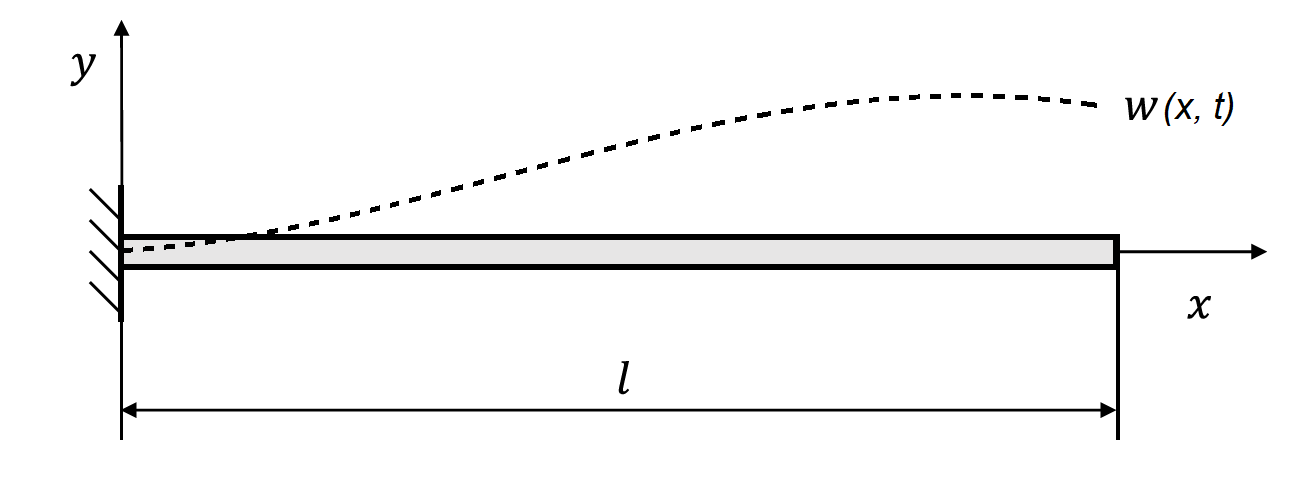
\includegraphics[width=0.6\textwidth]{figures/verification/linear-continuous-beam.png}
\caption{Linear, continuous cantilever beam}
\label{fig:verification:linear-continuous-beam}
\end{figure}

The solution for the free motion of the beam, without any external excitation, is found to be
%
\begin{align}
w(x,\,t) &= \sum_{i=1}^{\infty} W_{i}(x)H_{i}(t), \label{eq:linear-continuous-beam-w}
\end{align}

which is an infinite sum of mode shapes~$W_{i}(x)$, multiplied with harmonic oscillations~$H_{i}(t)$, each with a different natural frequency.
The shape functions depend on the boundary conditions of the beam and are for this example given by
%
\begin{align}
W_{i}(x) &= \cos(\kappa_{i}x) - \cosh(\kappa_{i}x) - \gamma_{i} \left( \sin(\kappa_{i}x) - \sinh(\kappa_{i}x) \right) \\
\gamma_{i} &= \frac{\cos(\kappa_{i}l) + \cosh(\kappa_{i}l)}{\sin(\kappa_{i}l) + \sinh(\kappa_{i}l)} \notag
\end{align}

with the constants $\kappa_{i}$ being approximately determined by    % https://wandinger.userweb.mwn.de/LA_Elastodynamik_2/kap_3_balken.pdf
%
\begin{align}
\kappa_{1}l &\approx 1.8751,\ \kappa_{2}l \approx 4.6941,\ \kappa_{3}l\ \approx 7.8548,\ \kappa_{4}l \approx 10.996, \\
\kappa_{i}l &\approx (2i - 1)\frac{\pi}{2}\ \ \mathrm{for}\ \ i > 4. \notag
\end{align}

The time-dependent functions $H_{i}(t)$ with the eigenfrequencies $\omega_{i}$ and free constants $A_{i}$ and $B_{i}$ are
%
\begin{equation}
H_{i}(t) = A_{i}\cos(\omega_{i}t) + B_{i}\sin(\omega_{i}t),\quad \omega_{i} = \kappa_{i}^2 \sqrt{\frac{EI}{\rho A}}.
\end{equation}

The constants can be determined from the initial conditions of the beam, i.e. the initial displacement $w(x,\,0) = w_{0}(x)$ and velocity $\dot{w}(x,\,0) = v_{0}(x)$,
%
\begin{align}
A_{i} &= \frac{1}{l}\int_{0}^{l} w_{0}(x)W_{i}(x) dx, \\
B_{i} &= \frac{1}{\omega_{i}l}\int_{0}^{l} v_{0}(x)W_{i}(x) dx.
\end{align}

With these equations the motion of the beam in space and time can be computed up to an arbitrary accuracy by including as many modes and natural frequencies as required.